\section{Our Approach ArchRAG}
\label{sec:ArchRAG}

Unlike GraphRAG, which purely uses links to generate communities, we propose to detect communities that can be organized into a hierarchical tree structure by exploiting both links and attributes in the knowledge graph, also called attributed communities.
%
An attributed community is a group of entities with a summary, where the entities are not only densely connected but also share similar themes, providing detailed information for answering specific questions, and the summary can offer a condensed view for answering abstract questions since it enables more focused engagement with the entities’ attributes.
%
Moreover, in the hierarchical tree structure, the lower-level communities and entities contain detailed knowledge from the KG, while higher-level communities provide global summaries, which naturally enable ArchRAG to address questions with different granularity in abstraction.

Moreover, to answer questions, we need to efficiently identify highly relevant attributed communities at different levels of the hierarchical structure.
% 
Considering that our hierarchical attributed communities and the HNSW index~\cite{malkov2018efficient} are similar in structure, we propose to map entities and attributed communities into high-dimensional nodes and then build a unified Community-based HNSW (C-HNSW) index for them, which allows us to efficiently identify the highly relevant attributed communities.

As illustrated in Figure~\ref{fig:overview}, our proposed ArchRAG consists of two phases. 
% 
In the {\it offline indexing} phase, ArchRAG first constructs a KG from the corpus, then detects attributed communities by a novel LLM-based hierarchical clustering method, and finally builds the C-HNSW index.
% Subsequently, to enable efficient retrieval, we propose a unified Community-based HNSW (C-HNSW) index to hierarchically organize both the attributed communities and entities, each of which is mapped into a high-dimensional vector.
% 
During the {\it online retrieval} phase, ArchRAG first converts the question into a query vector, then retrieves relevant information from the C-HNSW index, and finally generates answers through adaptive filtering-based generation process which identifies the most relevant information.

% 
%To avoid overwhelming the LLM with excessive retrieved information (e.g., the ``lost in the middle'' dilemma~\cite{liu2024lost}), we propose an adaptive filtering generation approach that first analyzes each retrieved information, then filters the content based on relevance, and finally generates the final response using the refined information.

% By efficiently searching and integrating retrieved information across various granularities, ArchRAG is highly cost-efficient and adaptable to questions of different levels of detail, namely, both specific and abstract questions.
%


% As illustrated in Figure~\ref{fig:overview}, our proposed ArchRAG also consists of two phases: {\it offline indexing} and {\it online retrieval}. 
% % 
% In the {\it offline indexing} phase, ArchRAG first constructs a KG by using LLM to extract entities and relationships from the corpus, and then detects attributed communities by a novel LLM-based hierarchical clustering method.
% %
% Subsequently, to enable efficient retrieval, we propose a unified Community-based HNSW (C-HNSW) index to hierarchically organize both the attributed communities and entities, each of which is mapped into a high-dimensional vector.

% During the {\it online retrieval} phase, ArchRAG first converts the question into a query vector, and then retrieve relevant information from the C-HNSW index by an efficient hierarchical search.
% % 
% To avoid overwhelming the LLM with excessive retrieved information (i.e., the ``lost in the middle'' dilemma~\cite{liu2024lost}), we propose an adaptive filtering generation approach that leverages LLM analysis to integrate the retrieved information, which first analyzes each retrieved information, filters the content based on relevance, and subsequently generates the final response using the refined information.
% % 
% By efficiently searching and integrating retrieved information across various granularities, ArchRAG is highly cost-efficient and adaptable to questions of different levels of detail, namely, both specific and abstract questions.
% %
% Next, we introduce the details of both offline and online phases of ArchRAG.

\section{Experiments} \label{sec:experiments}

\section{Dataset}
\label{sec:dataset}

\subsection{Data Collection}

To analyze political discussions on Discord, we followed the methodology in \cite{singh2024Cross-Platform}, collecting messages from politically-oriented public servers in compliance with Discord's platform policies.

Using Discord's Discovery feature, we employed a web scraper to extract server invitation links, names, and descriptions, focusing on public servers accessible without participation. Invitation links were used to access data via the Discord API. To ensure relevance, we filtered servers using keywords related to the 2024 U.S. elections (e.g., Trump, Kamala, MAGA), as outlined in \cite{balasubramanian2024publicdatasettrackingsocial}. This resulted in 302 server links, further narrowed to 81 English-speaking, politics-focused servers based on their names and descriptions.

Public messages were retrieved from these servers using the Discord API, collecting metadata such as \textit{content}, \textit{user ID}, \textit{username}, \textit{timestamp}, \textit{bot flag}, \textit{mentions}, and \textit{interactions}. Through this process, we gathered \textbf{33,373,229 messages} from \textbf{82,109 users} across \textbf{81 servers}, including \textbf{1,912,750 messages} from \textbf{633 bots}. Data collection occurred between November 13th and 15th, covering messages sent from January 1st to November 12th, just after the 2024 U.S. election.

\subsection{Characterizing the Political Spectrum}
\label{sec:timeline}

A key aspect of our research is distinguishing between Republican- and Democratic-aligned Discord servers. To categorize their political alignment, we relied on server names and self-descriptions, which often include rules, community guidelines, and references to key ideologies or figures. Each server's name and description were manually reviewed based on predefined, objective criteria, focusing on explicit political themes or mentions of prominent figures. This process allowed us to classify servers into three categories, ensuring a systematic and unbiased alignment determination.

\begin{itemize}
    \item \textbf{Republican-aligned}: Servers referencing Republican and right-wing and ideologies, movements, or figures (e.g., MAGA, Conservative, Traditional, Trump).  
    \item \textbf{Democratic-aligned}: Servers mentioning Democratic and left-wing ideologies, movements, or figures (e.g., Progressive, Liberal, Socialist, Biden, Kamala).  
    \item \textbf{Unaligned}: Servers with no defined spectrum and ideologies or opened to general political debate from all orientations.
\end{itemize}

To ensure the reliability and consistency of our classification, three independent reviewers assessed the classification following the specified set of criteria. The inter-rater agreement of their classifications was evaluated using Fleiss' Kappa \cite{fleiss1971measuring}, with a resulting Kappa value of \( 0.8191 \), indicating an almost perfect agreement among the reviewers. Disagreements were resolved by adopting the majority classification, as there were no instances where a server received different classifications from all three reviewers. This process guaranteed the consistency and accuracy of the final categorization.

Through this process, we identified \textbf{7 Republican-aligned servers}, \textbf{9 Democratic-aligned servers}, and \textbf{65 unaligned servers}.

Table \ref{tab:statistics} shows the statistics of the collected data. Notably, while Democratic- and Republican-aligned servers had a comparable number of user messages, users in the latter servers were significantly more active, posting more than double the number of messages per user compared to their Democratic counterparts. 
This suggests that, in our sample, Democratic-aligned servers attract more users, but these users were less engaged in text-based discussions. Additionally, around 10\% of the messages across all server categories were posted by bots. 

\subsection{Temporal Data} 

Throughout this paper, we refer to the election candidates using the names adopted by their respective campaigns: \textit{Kamala}, \textit{Biden}, and \textit{Trump}. To examine how the content of text messages evolves based on the political alignment of servers, we divided the 2024 election year into three periods: \textbf{Biden vs Trump} (January 1 to July 21), \textbf{Kamala vs Trump} (July 21 to September 20), and the \textbf{Voting Period} (after September 20). These periods reflect key phases of the election: the early campaign dominated by Biden and Trump, the shift in dynamics with Kamala Harris replacing Joe Biden as the Democratic candidate, and the final voting stage focused on electoral outcomes and their implications. This segmentation enables an analysis of how discourse responds to pivotal electoral moments.

Figure \ref{fig:line-plot} illustrates the distribution of messages over time, highlighting trends in total messages volume and mentions of each candidate. Prior to Biden's withdrawal on July 21, mentions of Biden and Trump were relatively balanced. However, following Kamala's entry into the race, mentions of Trump surged significantly, a trend further amplified by an assassination attempt on him, solidifying his dominance in the discourse. The only instance where Trump’s mentions were exceeded occurred during the first debate, as concerns about Biden’s age and cognitive abilities temporarily shifted the focus. In the final stages of the election, mentions of all three candidates rose, with Trump’s mentions peaking as he emerged as the victor.

\definecolor{darkgreen}{rgb}{0.0, 0.5, 0.0}
\definecolor{violet}{rgb}{0.56, 0.0, 1.0}
\section{Evaluation}
We apply our methodology to derive counterfactual policies for various MDPs, addressing three main research questions: (1) how does our policy's performance compare to the Gumbel-max SCM approach; (2) how do the counterfactual stability and monotonicity assumptions impact the probability bounds; and (3) how fast is our approach compared with the Gumbel-max SCM method?

\begin{figure*}
    \centering
    %
    \resizebox{0.6\textwidth}{!}{
        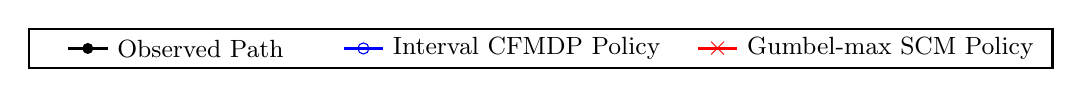
\begin{tikzpicture}[scale=1.0, every node/.style={scale=1.0}]
            \draw[thick, black] (-3, -0.25) rectangle (10, 0.25);
            %
            \draw[black, line width=1pt] (-2.5, 0.0) -- (-2,0.0);
            \fill[black] (-2.25,0.0) circle (2pt); %
            \node[right] at (-2,0.0) {\small Observed Path};
            
            %
            \draw[blue, line width=1pt] (1.0,0.0) -- (1.5,0.0);
            \node[draw=blue, circle, minimum size=4pt, inner sep=0pt] at (1.25,0.0) {}; %
            \node[right] at (1.5,0.0) {\small Interval CFMDP Policy};
            
            %
            \draw[red, line width=1pt] (5.5,0) -- (6,0);
            \node[red] at (5.75,0) {$\boldsymbol{\times}$}; %
            \node[right] at (6,0) {\small Gumbel-max SCM Policy};
        \end{tikzpicture}
    }\\
    %
    \subfigure[\footnotesize Lowest cumulative reward: Interval CFMDP ($312$), Gumbel-max SCM ($312$)]{%
        \resizebox{0.76\columnwidth}{!}{
             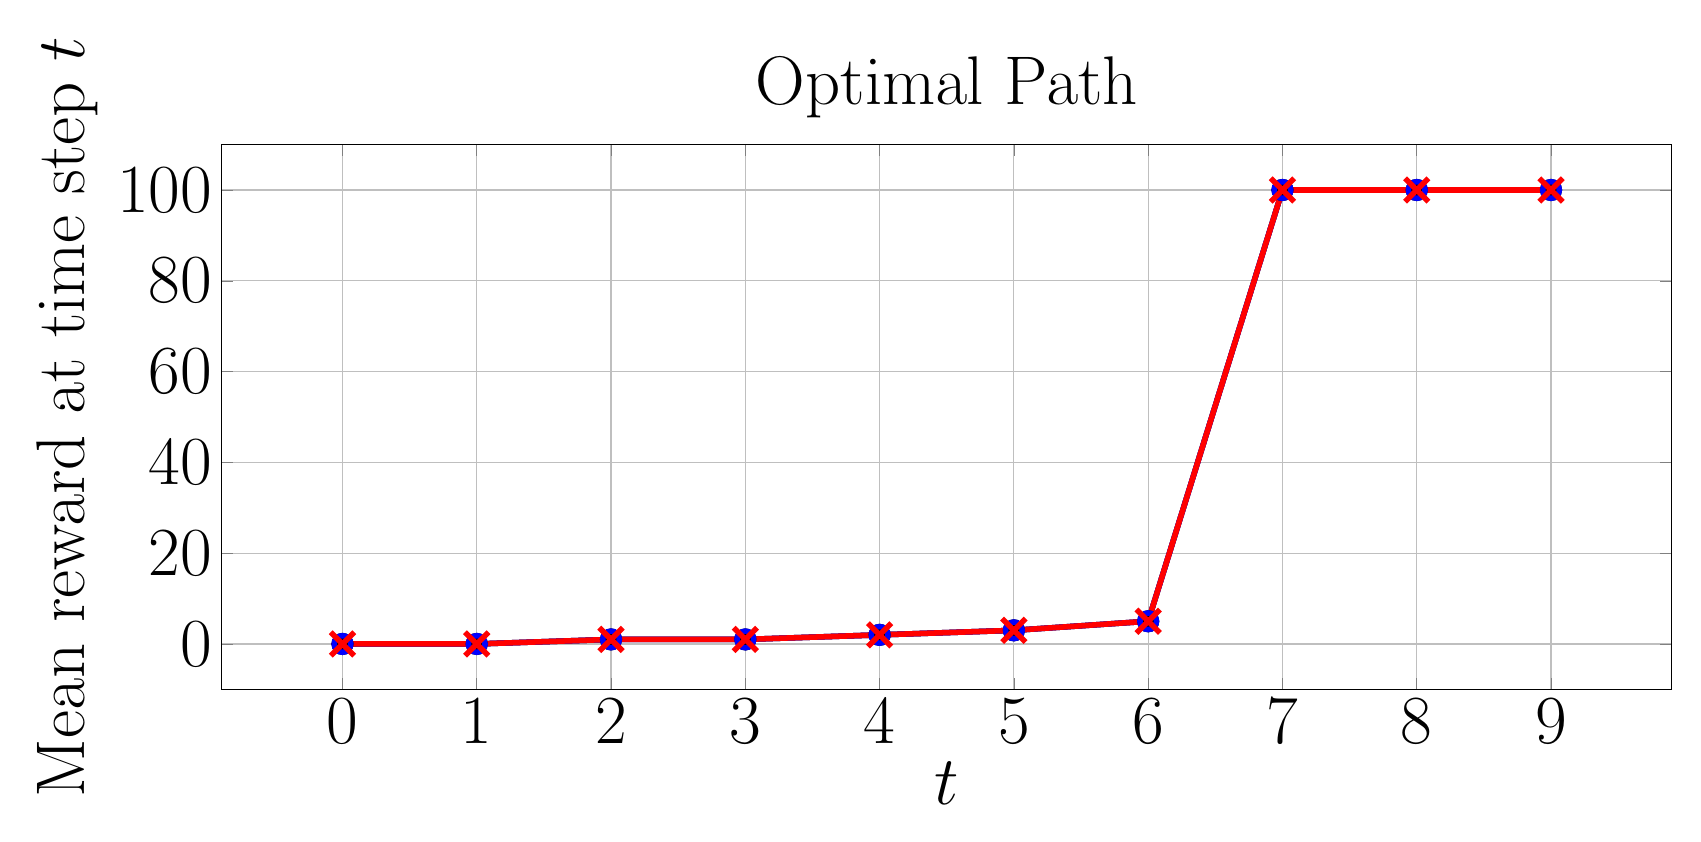
\begin{tikzpicture}
                \begin{axis}[
                    xlabel={$t$},
                    ylabel={Mean reward at time step $t$},
                    title={Optimal Path},
                    grid=both,
                    width=20cm, height=8.5cm,
                    every axis/.style={font=\Huge},
                    %
                ]
                \addplot[
                    color=black, %
                    mark=*, %
                    line width=2pt,
                    mark size=3pt,
                    error bars/.cd,
                    y dir=both, %
                    y explicit, %
                    error bar style={line width=1pt,solid},
                    error mark options={line width=1pt,mark size=4pt,rotate=90}
                ]
                coordinates {
                    (0, 0.0)  +- (0, 0.0)
                    (1, 0.0)  +- (0, 0.0) 
                    (2, 1.0)  +- (0, 0.0) 
                    (3, 1.0)  +- (0, 0.0)
                    (4, 2.0)  +- (0, 0.0)
                    (5, 3.0) +- (0, 0.0)
                    (6, 5.0) +- (0, 0.0)
                    (7, 100.0) +- (0, 0.0)
                    (8, 100.0) +- (0, 0.0)
                    (9, 100.0) +- (0, 0.0)
                };
                %
                \addplot[
                    color=blue, %
                    mark=o, %
                    line width=2pt,
                    mark size=3pt,
                    error bars/.cd,
                    y dir=both, %
                    y explicit, %
                    error bar style={line width=1pt,solid},
                    error mark options={line width=1pt,mark size=4pt,rotate=90}
                ]
                 coordinates {
                    (0, 0.0)  +- (0, 0.0)
                    (1, 0.0)  +- (0, 0.0) 
                    (2, 1.0)  +- (0, 0.0) 
                    (3, 1.0)  +- (0, 0.0)
                    (4, 2.0)  +- (0, 0.0)
                    (5, 3.0) +- (0, 0.0)
                    (6, 5.0) +- (0, 0.0)
                    (7, 100.0) +- (0, 0.0)
                    (8, 100.0) +- (0, 0.0)
                    (9, 100.0) +- (0, 0.0)
                };
                %
                \addplot[
                    color=red, %
                    mark=x, %
                    line width=2pt,
                    mark size=6pt,
                    error bars/.cd,
                    y dir=both, %
                    y explicit, %
                    error bar style={line width=1pt,solid},
                    error mark options={line width=1pt,mark size=4pt,rotate=90}
                ]
                coordinates {
                    (0, 0.0)  +- (0, 0.0)
                    (1, 0.0)  +- (0, 0.0) 
                    (2, 1.0)  +- (0, 0.0) 
                    (3, 1.0)  +- (0, 0.0)
                    (4, 2.0)  +- (0, 0.0)
                    (5, 3.0) +- (0, 0.0)
                    (6, 5.0) +- (0, 0.0)
                    (7, 100.0) +- (0, 0.0)
                    (8, 100.0) +- (0, 0.0)
                    (9, 100.0) +- (0, 0.0)
                };
                \end{axis}
            \end{tikzpicture}
         }
    }
    \hspace{1cm}
    \subfigure[\footnotesize Lowest cumulative reward: Interval CFMDP ($19$), Gumbel-max SCM ($-88$)]{%
         \resizebox{0.76\columnwidth}{!}{
            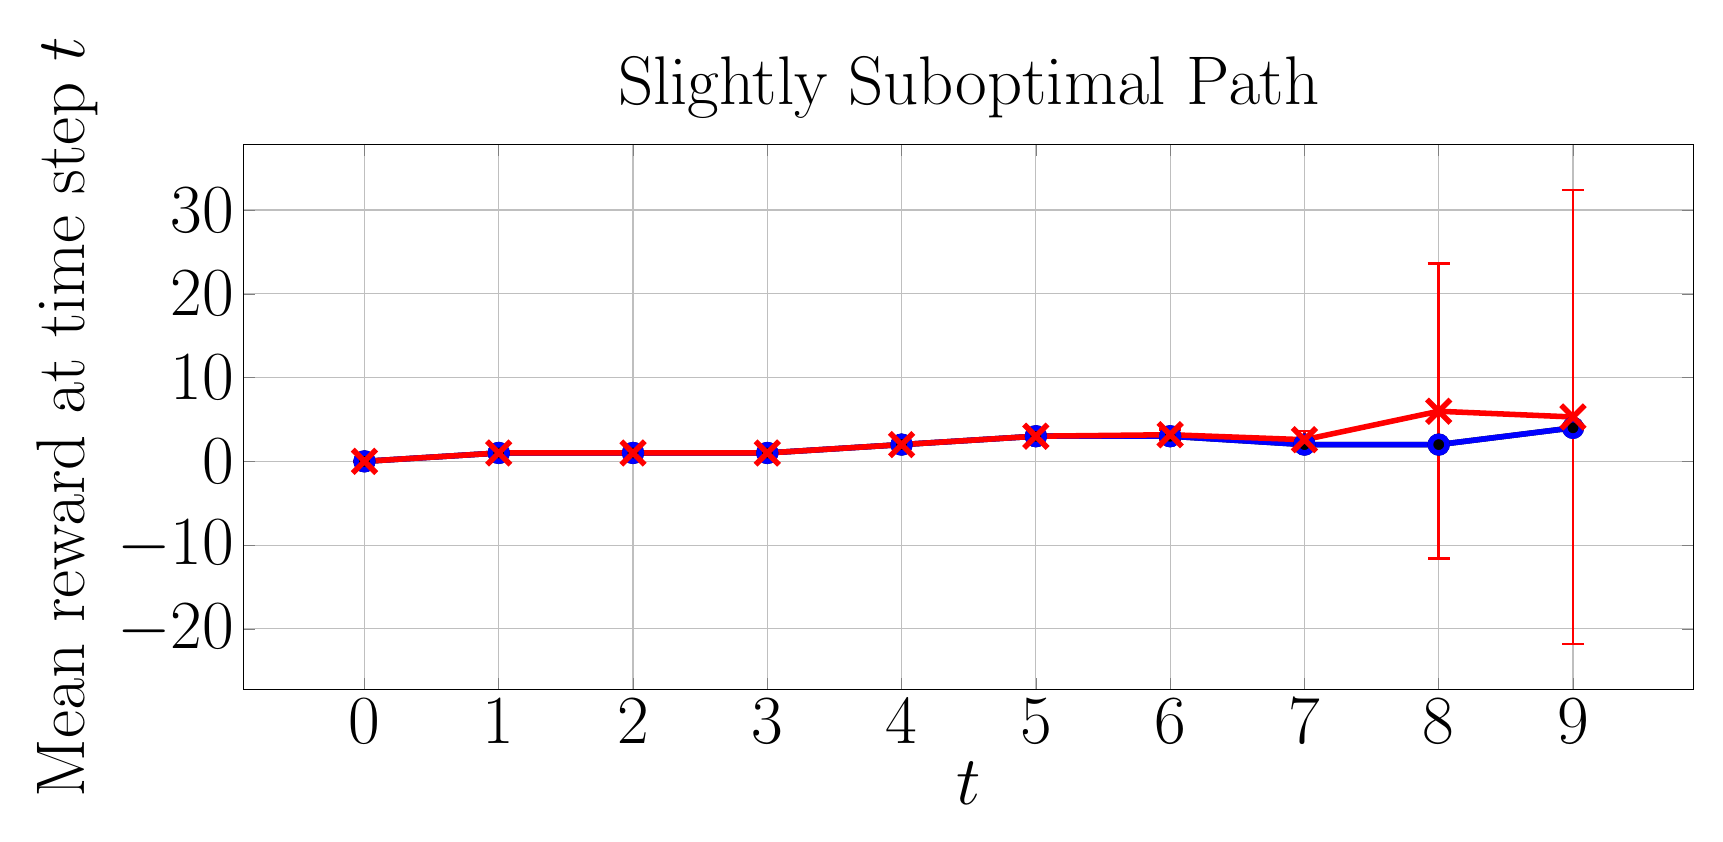
\begin{tikzpicture}
                \begin{axis}[
                    xlabel={$t$},
                    ylabel={Mean reward at time step $t$},
                    title={Slightly Suboptimal Path},
                    grid=both,
                    width=20cm, height=8.5cm,
                    every axis/.style={font=\Huge},
                    %
                ]
                \addplot[
                    color=black, %
                    mark=*, %
                    line width=2pt,
                    mark size=3pt,
                    error bars/.cd,
                    y dir=both, %
                    y explicit, %
                    error bar style={line width=1pt,solid},
                    error mark options={line width=1pt,mark size=4pt,rotate=90}
                ]
              coordinates {
                    (0, 0.0)  +- (0, 0.0)
                    (1, 1.0)  +- (0, 0.0) 
                    (2, 1.0)  +- (0, 0.0) 
                    (3, 1.0)  +- (0, 0.0)
                    (4, 2.0)  +- (0, 0.0)
                    (5, 3.0) +- (0, 0.0)
                    (6, 3.0) +- (0, 0.0)
                    (7, 2.0) +- (0, 0.0)
                    (8, 2.0) +- (0, 0.0)
                    (9, 4.0) +- (0, 0.0)
                };
                %
                \addplot[
                    color=blue, %
                    mark=o, %
                    line width=2pt,
                    mark size=3pt,
                    error bars/.cd,
                    y dir=both, %
                    y explicit, %
                    error bar style={line width=1pt,solid},
                    error mark options={line width=1pt,mark size=4pt,rotate=90}
                ]
              coordinates {
                    (0, 0.0)  +- (0, 0.0)
                    (1, 1.0)  +- (0, 0.0) 
                    (2, 1.0)  +- (0, 0.0) 
                    (3, 1.0)  +- (0, 0.0)
                    (4, 2.0)  +- (0, 0.0)
                    (5, 3.0) +- (0, 0.0)
                    (6, 3.0) +- (0, 0.0)
                    (7, 2.0) +- (0, 0.0)
                    (8, 2.0) +- (0, 0.0)
                    (9, 4.0) +- (0, 0.0)
                };
                %
                \addplot[
                    color=red, %
                    mark=x, %
                    line width=2pt,
                    mark size=6pt,
                    error bars/.cd,
                    y dir=both, %
                    y explicit, %
                    error bar style={line width=1pt,solid},
                    error mark options={line width=1pt,mark size=4pt,rotate=90}
                ]
                coordinates {
                    (0, 0.0)  +- (0, 0.0)
                    (1, 1.0)  +- (0, 0.0) 
                    (2, 1.0)  +- (0, 0.0) 
                    (3, 1.0)  +- (0, 0.0)
                    (4, 2.0)  += (0, 0.0)
                    (5, 3.0)  += (0, 0.0)
                    (6, 3.17847) += (0, 0.62606746) -= (0, 0.62606746)
                    (7, 2.5832885) += (0, 1.04598233) -= (0, 1.04598233)
                    (8, 5.978909) += (0, 17.60137623) -= (0, 17.60137623)
                    (9, 5.297059) += (0, 27.09227512) -= (0, 27.09227512)
                };
                \end{axis}
            \end{tikzpicture}
         }
    }\\[-1.5pt]
    \subfigure[\footnotesize Lowest cumulative reward: Interval CFMDP ($14$), Gumbel-max SCM ($-598$)]{%
         \resizebox{0.76\columnwidth}{!}{
             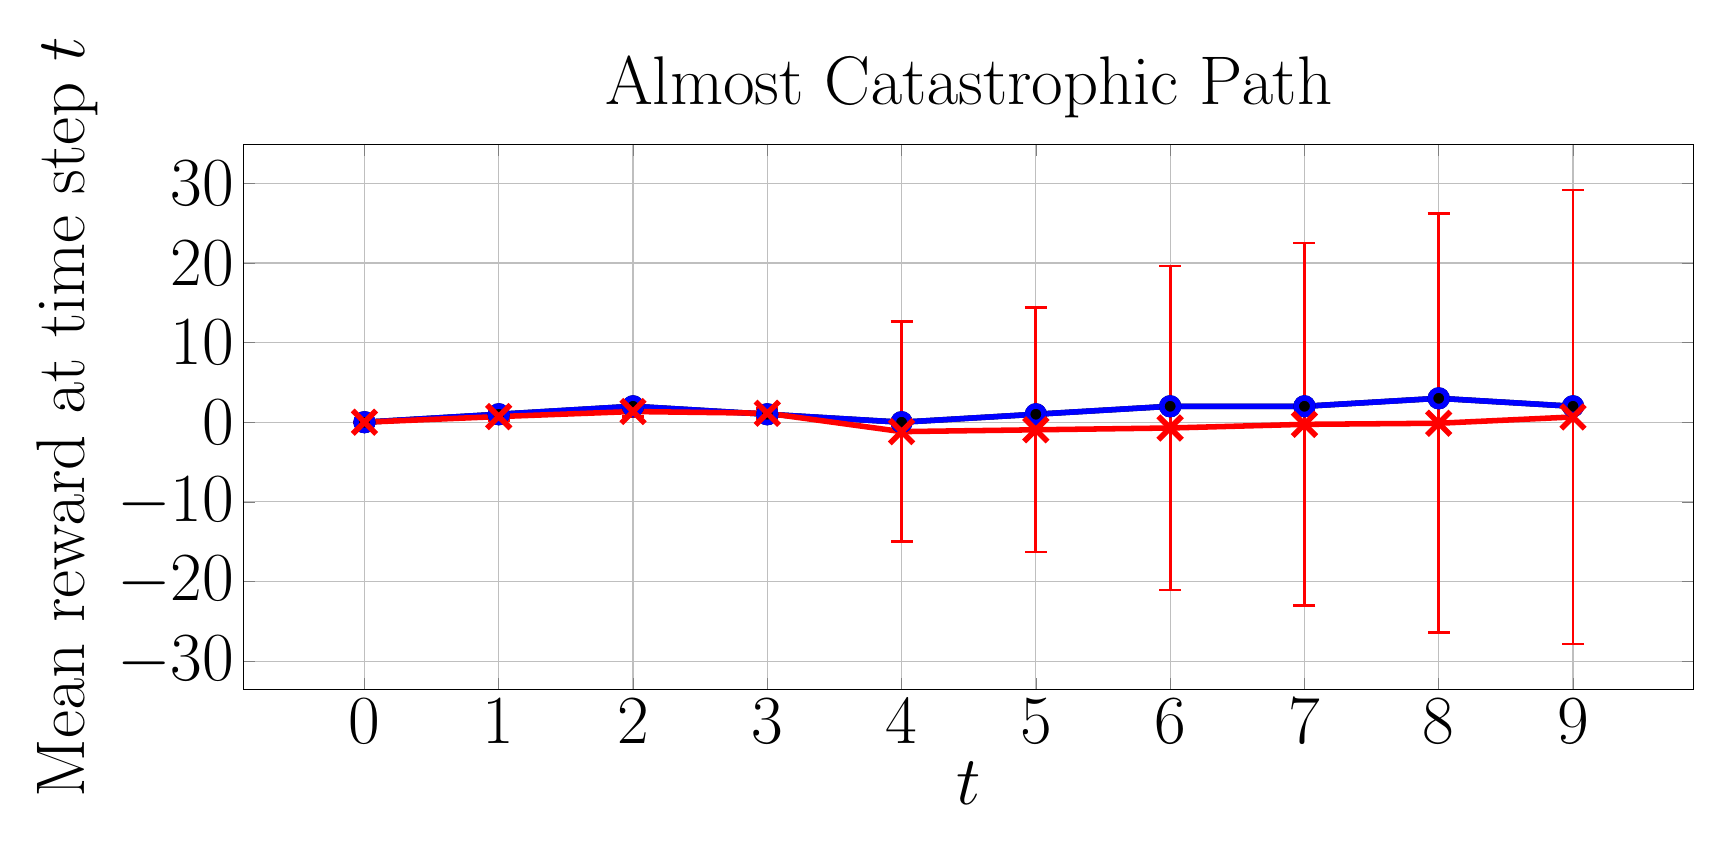
\begin{tikzpicture}
                \begin{axis}[
                    xlabel={$t$},
                    ylabel={Mean reward at time step $t$},
                    title={Almost Catastrophic Path},
                    grid=both,
                    width=20cm, height=8.5cm,
                    every axis/.style={font=\Huge},
                    %
                ]
                \addplot[
                    color=black, %
                    mark=*, %
                    line width=2pt,
                    mark size=3pt,
                    error bars/.cd,
                    y dir=both, %
                    y explicit, %
                    error bar style={line width=1pt,solid},
                    error mark options={line width=1pt,mark size=4pt,rotate=90}
                ]
                coordinates {
                    (0, 0.0)  +- (0, 0.0)
                    (1, 1.0)  +- (0, 0.0) 
                    (2, 2.0)  +- (0, 0.0) 
                    (3, 1.0)  +- (0, 0.0)
                    (4, 0.0)  +- (0, 0.0)
                    (5, 1.0) +- (0, 0.0)
                    (6, 2.0) +- (0, 0.0)
                    (7, 2.0) +- (0, 0.0)
                    (8, 3.0) +- (0, 0.0)
                    (9, 2.0) +- (0, 0.0)
                };
                %
                \addplot[
                    color=blue, %
                    mark=o, %
                    line width=2pt,
                    mark size=3pt,
                    error bars/.cd,
                    y dir=both, %
                    y explicit, %
                    error bar style={line width=1pt,solid},
                    error mark options={line width=1pt,mark size=4pt,rotate=90}
                ]
                coordinates {
                    (0, 0.0)  +- (0, 0.0)
                    (1, 1.0)  +- (0, 0.0) 
                    (2, 2.0)  +- (0, 0.0) 
                    (3, 1.0)  +- (0, 0.0)
                    (4, 0.0)  +- (0, 0.0)
                    (5, 1.0) +- (0, 0.0)
                    (6, 2.0) +- (0, 0.0)
                    (7, 2.0) +- (0, 0.0)
                    (8, 3.0) +- (0, 0.0)
                    (9, 2.0) +- (0, 0.0)
                };
                %
                \addplot[
                    color=red, %
                    mark=x, %
                    line width=2pt,
                    mark size=6pt,
                    error bars/.cd,
                    y dir=both, %
                    y explicit, %
                    error bar style={line width=1pt,solid},
                    error mark options={line width=1pt,mark size=4pt,rotate=90}
                ]
                coordinates {
                    (0, 0.0)  +- (0, 0.0)
                    (1, 0.7065655)  +- (0, 0.4553358) 
                    (2, 1.341673)  +- (0, 0.67091621) 
                    (3, 1.122926)  +- (0, 0.61281824)
                    (4, -1.1821935)  +- (0, 13.82444042)
                    (5, -0.952399)  +- (0, 15.35195457)
                    (6, -0.72672) +- (0, 20.33508414)
                    (7, -0.268983) +- (0, 22.77861454)
                    (8, -0.1310835) +- (0, 26.31013314)
                    (9, 0.65806) +- (0, 28.50670214)
                };
                %
            %
            %
            %
            %
            %
            %
            %
            %
            %
            %
            %
            %
            %
            %
            %
            %
            %
            %
                \end{axis}
            \end{tikzpicture}
         }
    }
    \hspace{1cm}
    \subfigure[\footnotesize Lowest cumulative reward: Interval CFMDP ($-698$), Gumbel-max SCM ($-698$)]{%
         \resizebox{0.76\columnwidth}{!}{
            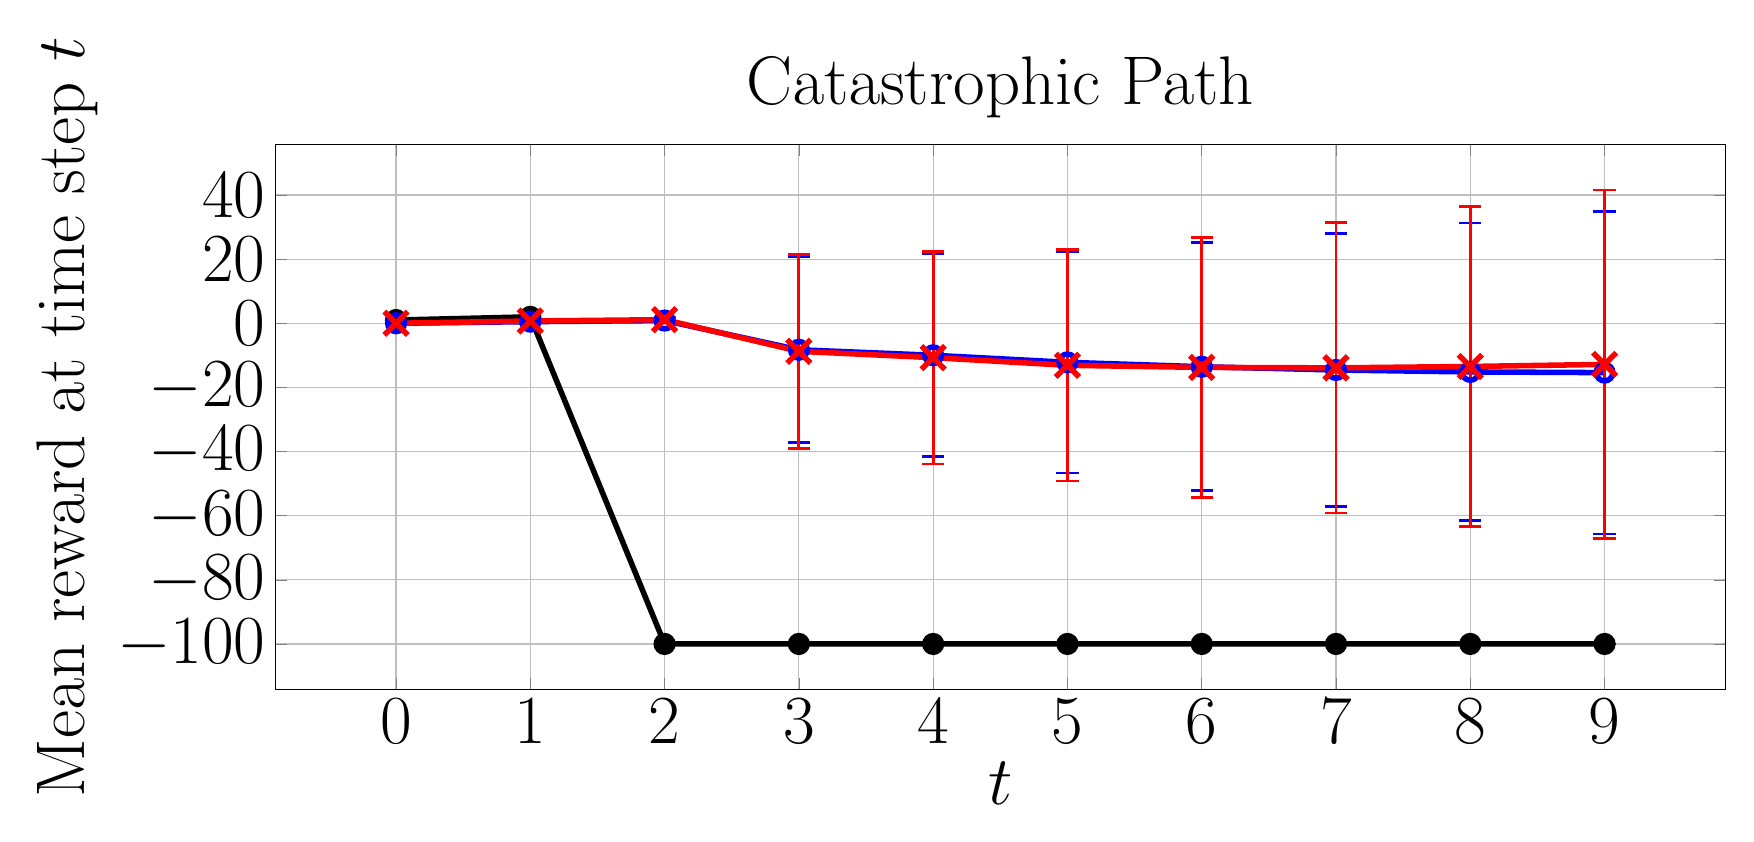
\begin{tikzpicture}
                \begin{axis}[
                    xlabel={$t$},
                    ylabel={Mean reward at time step $t$},
                    title={Catastrophic Path},
                    grid=both,
                    width=20cm, height=8.5cm,
                    every axis/.style={font=\Huge},
                    %
                ]
                \addplot[
                    color=black, %
                    mark=*, %
                    line width=2pt,
                    mark size=3pt,
                    error bars/.cd,
                    y dir=both, %
                    y explicit, %
                    error bar style={line width=1pt,solid},
                    error mark options={line width=1pt,mark size=4pt,rotate=90}
                ]
                coordinates {
                    (0, 1.0)  +- (0, 0.0)
                    (1, 2.0)  +- (0, 0.0) 
                    (2, -100.0)  +- (0, 0.0) 
                    (3, -100.0)  +- (0, 0.0)
                    (4, -100.0)  +- (0, 0.0)
                    (5, -100.0) +- (0, 0.0)
                    (6, -100.0) +- (0, 0.0)
                    (7, -100.0) +- (0, 0.0)
                    (8, -100.0) +- (0, 0.0)
                    (9, -100.0) +- (0, 0.0)
                };
                %
                \addplot[
                    color=blue, %
                    mark=o, %
                    line width=2pt,
                    mark size=3pt,
                    error bars/.cd,
                    y dir=both, %
                    y explicit, %
                    error bar style={line width=1pt,solid},
                    error mark options={line width=1pt,mark size=4pt,rotate=90}
                ]
                coordinates {
                    (0, 0.0)  +- (0, 0.0)
                    (1, 0.504814)  +- (0, 0.49997682) 
                    (2, 0.8439835)  +- (0, 0.76831917) 
                    (3, -8.2709165)  +- (0, 28.93656754)
                    (4, -9.981082)  +- (0, 31.66825363)
                    (5, -12.1776325) +- (0, 34.53463233)
                    (6, -13.556076) +- (0, 38.62845372)
                    (7, -14.574418) +- (0, 42.49603359)
                    (8, -15.1757075) +- (0, 46.41913968)
                    (9, -15.3900395) +- (0, 50.33563368)
                };
                %
                \addplot[
                    color=red, %
                    mark=x, %
                    line width=2pt,
                    mark size=6pt,
                    error bars/.cd,
                    y dir=both, %
                    y explicit, %
                    error bar style={line width=1pt,solid},
                    error mark options={line width=1pt,mark size=4pt,rotate=90}
                ]
                coordinates {
                    (0, 0.0)  +- (0, 0.0)
                    (1, 0.701873)  +- (0, 0.45743556) 
                    (2, 1.1227805)  +- (0, 0.73433129) 
                    (3, -8.7503255)  +- (0, 30.30257976)
                    (4, -10.722092)  +- (0, 33.17618589)
                    (5, -13.10721)  +- (0, 36.0648089)
                    (6, -13.7631645) +- (0, 40.56553451)
                    (7, -13.909043) +- (0, 45.23829402)
                    (8, -13.472517) +- (0, 49.96270296)
                    (9, -12.8278835) +- (0, 54.38618735)
                };
                %
            %
            %
            %
            %
            %
            %
            %
            %
            %
            %
            %
            %
            %
            %
            %
            %
            %
            %
                \end{axis}
            \end{tikzpicture}
         }
    }
    \caption{Average instant reward of CF paths induced by policies on GridWorld $p=0.4$.}
    \label{fig: reward p=0.4}
\end{figure*}

\subsection{Experimental Setup}
To compare policy performance, we measure the average rewards of counterfactual paths induced by our policy and the Gumbel-max policy by uniformly sampling $200$ counterfactual MDPs from the ICFMDP and generating $10,000$ counterfactual paths over each sampled CFMDP. \jl{Since the interval CFMDP depends on the observed path, we select $4$  paths of varying optimality to evaluate how the observed path impacts the performance of both policies: an optimal path, a slightly suboptimal path that could reach the optimal reward with a few changes, a catastrophic path that enters a catastrophic, terminal state with low reward, and an almost catastrophic path that was close to entering a catastrophic state.} When measuring the average probability bound widths and execution time needed to generate the ICFMDPs, we averaged over $20$ randomly generated observed paths
\footnote{Further training details are provided in Appendix \ref{app: training details}, and the code is provided at \href{https://github.com/ddv-lab/robust-cf-inference-in-MDPs}{https://github.com/ddv-lab/robust-cf-inference-in-MDPs}
%
%
.}.

\subsection{GridWorld}
\jl{The GridWorld MDP is a $4 \times 4$ grid where an agent must navigate from the top-left corner to the goal state in the bottom-right corner, avoiding a dangerous terminal state in the centre. At each time step, the agent can move up, down, left, or right, but there is a small probability (controlled by hyper-parameter $p$) of moving in an unintended direction. As the agent nears the goal, the reward for each state increases, culminating in a reward of $+100$ for reaching the goal. Entering the dangerous state results in a penalty of $-100$. We use two versions of GridWorld: a less stochastic version with $p=0.9$ (i.e., $90$\% chance of moving in the chosen direction) and a more stochastic version with $p=0.4$.}

\paragraph{GridWorld ($p=0.9$)}
When $p=0.9$, the counterfactual probability bounds are typically narrow (see Table \ref{tab:nonzero_probs} for average measurements). Consequently, as shown in Figure \ref{fig: reward p=0.9}, both policies are nearly identical and perform similarly well across the optimal, slightly suboptimal, and catastrophic paths.
%
However, for the almost catastrophic path, the interval CFMDP path is more conservative and follows the observed path more closely (as this is where the probability bounds are narrowest), which typically requires one additional step to reach the goal state than the Gumbel-max SCM policy.
%

\paragraph{GridWorld ($p=0.4$)}
\jl{When $p=0.4$, the GridWorld environment becomes more uncertain, increasing the risk of entering the dangerous state even if correct actions are chosen. Thus, as shown in Figure \ref{fig: reward p=0.4}, the interval CFMDP policy adopts a more conservative approach, avoiding deviation from the observed policy if it cannot guarantee higher counterfactual rewards (see the slightly suboptimal and almost catastrophic paths), whereas the Gumbel-max SCM is inconsistent: it can yield higher rewards, but also much lower rewards, reflected in the wide error bars.} For the catastrophic path, both policies must deviate from the observed path to achieve a higher reward and, in this case, perform similarly.
%
%
%
%
\subsection{Sepsis}
The Sepsis MDP \citep{oberst2019counterfactual} simulates trajectories of Sepsis patients. Each state consists of four vital signs (heart rate, blood pressure, oxygen concentration, and glucose levels), categorised as low, normal, or high.
and three treatments that can be toggled on/off at each time step (8 actions in total). Unlike \citet{oberst2019counterfactual}, we scale rewards based on the number of out-of-range vital signs, between $-1000$ (patient dies) and $1000$ (patient discharged). \jl{Like the GridWorld $p=0.4$ experiment, the Sepsis MDP is highly uncertain, as many states are equally likely to lead to optimal and poor outcomes. Thus, as shown in Figure \ref{fig: reward sepsis}, both policies follow the observed optimal and almost catastrophic paths to guarantee rewards are no worse than the observation.} However, improving the catastrophic path requires deviating from the observation. Here, the Gumbel-max SCM policy, on average, performs better than the interval CFMDP policy. But, since both policies have lower bounds clipped at $-1000$, neither policy reliably improves over the observation. In contrast, for the slightly suboptimal path, the interval CFMDP policy performs significantly better, shown by its higher lower bounds. 
Moreover, in these two cases, the worst-case counterfactual path generated by the interval CFMDP policy is better than that of the Gumbel-max SCM policy,
indicating its greater robustness.
%
\begin{figure*}
    \centering
     \resizebox{0.6\textwidth}{!}{
        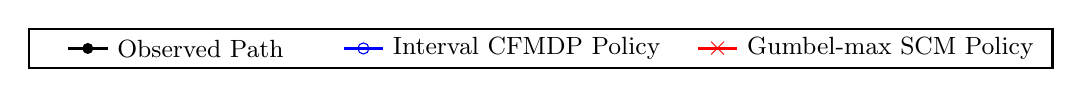
\begin{tikzpicture}[scale=1.0, every node/.style={scale=1.0}]
            \draw[thick, black] (-3, -0.25) rectangle (10, 0.25);
            %
            \draw[black, line width=1pt] (-2.5, 0.0) -- (-2,0.0);
            \fill[black] (-2.25,0.0) circle (2pt); %
            \node[right] at (-2,0.0) {\small Observed Path};
            
            %
            \draw[blue, line width=1pt] (1.0,0.0) -- (1.5,0.0);
            \node[draw=blue, circle, minimum size=4pt, inner sep=0pt] at (1.25,0.0) {}; %
            \node[right] at (1.5,0.0) {\small Interval CFMDP Policy};
            
            %
            \draw[red, line width=1pt] (5.5,0) -- (6,0);
            \node[red] at (5.75,0) {$\boldsymbol{\times}$}; %
            \node[right] at (6,0) {\small Gumbel-max SCM Policy};
        \end{tikzpicture}
    }\\
    \subfigure[\footnotesize Lowest cumulative reward: Interval CFMDP ($8000$), Gumbel-max SCM ($8000$)]{%
         \resizebox{0.76\columnwidth}{!}{
             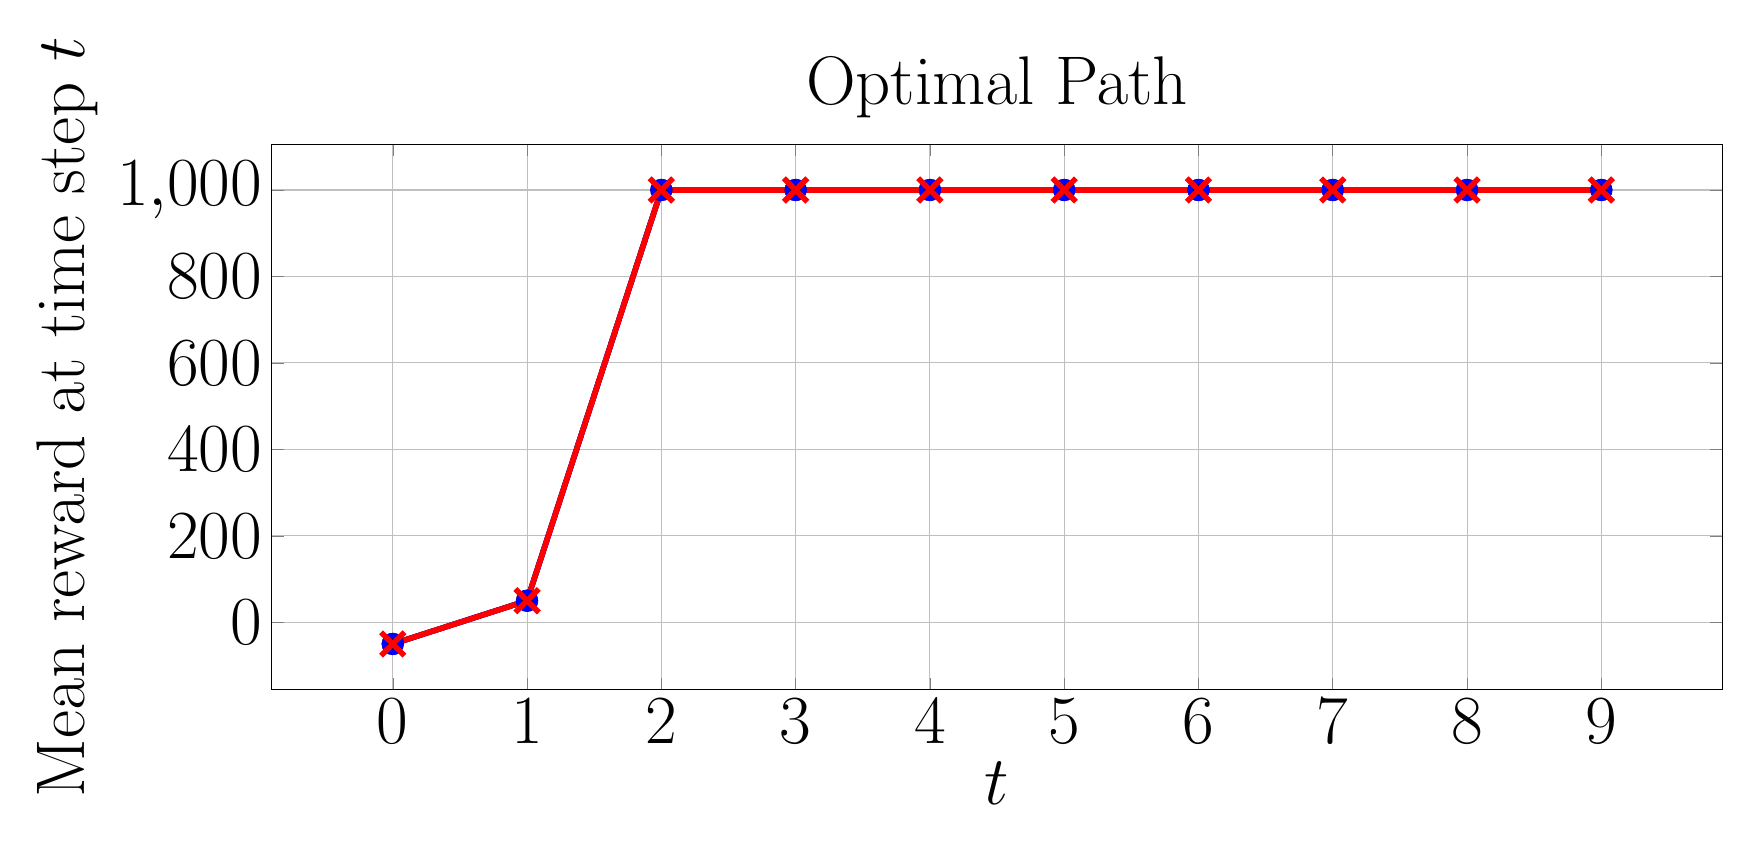
\begin{tikzpicture}
                \begin{axis}[
                    xlabel={$t$},
                    ylabel={Mean reward at time step $t$},
                    title={Optimal Path},
                    grid=both,
                    width=20cm, height=8.5cm,
                    every axis/.style={font=\Huge},
                    %
                ]
                \addplot[
                    color=black, %
                    mark=*, %
                    line width=2pt,
                    mark size=3pt,
                ]
                coordinates {
                    (0, -50.0)
                    (1, 50.0)
                    (2, 1000.0)
                    (3, 1000.0)
                    (4, 1000.0)
                    (5, 1000.0)
                    (6, 1000.0)
                    (7, 1000.0)
                    (8, 1000.0)
                    (9, 1000.0)
                };
                %
                \addplot[
                    color=blue, %
                    mark=o, %
                    line width=2pt,
                    mark size=3pt,
                    error bars/.cd,
                    y dir=both, %
                    y explicit, %
                    error bar style={line width=1pt,solid},
                    error mark options={line width=1pt,mark size=4pt,rotate=90}
                ]
                coordinates {
                    (0, -50.0)  +- (0, 0.0)
                    (1, 50.0)  +- (0, 0.0) 
                    (2, 1000.0)  +- (0, 0.0) 
                    (3, 1000.0)  +- (0, 0.0)
                    (4, 1000.0)  +- (0, 0.0)
                    (5, 1000.0) +- (0, 0.0)
                    (6, 1000.0) +- (0, 0.0)
                    (7, 1000.0) +- (0, 0.0)
                    (8, 1000.0) +- (0, 0.0)
                    (9, 1000.0) +- (0, 0.0)
                };
                %
                \addplot[
                    color=red, %
                    mark=x, %
                    line width=2pt,
                    mark size=6pt,
                    error bars/.cd,
                    y dir=both, %
                    y explicit, %
                    error bar style={line width=1pt,solid},
                    error mark options={line width=1pt,mark size=4pt,rotate=90}
                ]
                coordinates {
                    (0, -50.0)  +- (0, 0.0)
                    (1, 50.0)  +- (0, 0.0) 
                    (2, 1000.0)  +- (0, 0.0) 
                    (3, 1000.0)  +- (0, 0.0)
                    (4, 1000.0)  +- (0, 0.0)
                    (5, 1000.0) +- (0, 0.0)
                    (6, 1000.0) +- (0, 0.0)
                    (7, 1000.0) +- (0, 0.0)
                    (8, 1000.0) +- (0, 0.0)
                    (9, 1000.0) +- (0, 0.0)
                };
                %
                \end{axis}
            \end{tikzpicture}
         }
    }
    \hspace{1cm}
    \subfigure[\footnotesize Lowest cumulative reward: Interval CFMDP ($-5980$), Gumbel-max SCM ($-8000$)]{%
         \resizebox{0.76\columnwidth}{!}{
            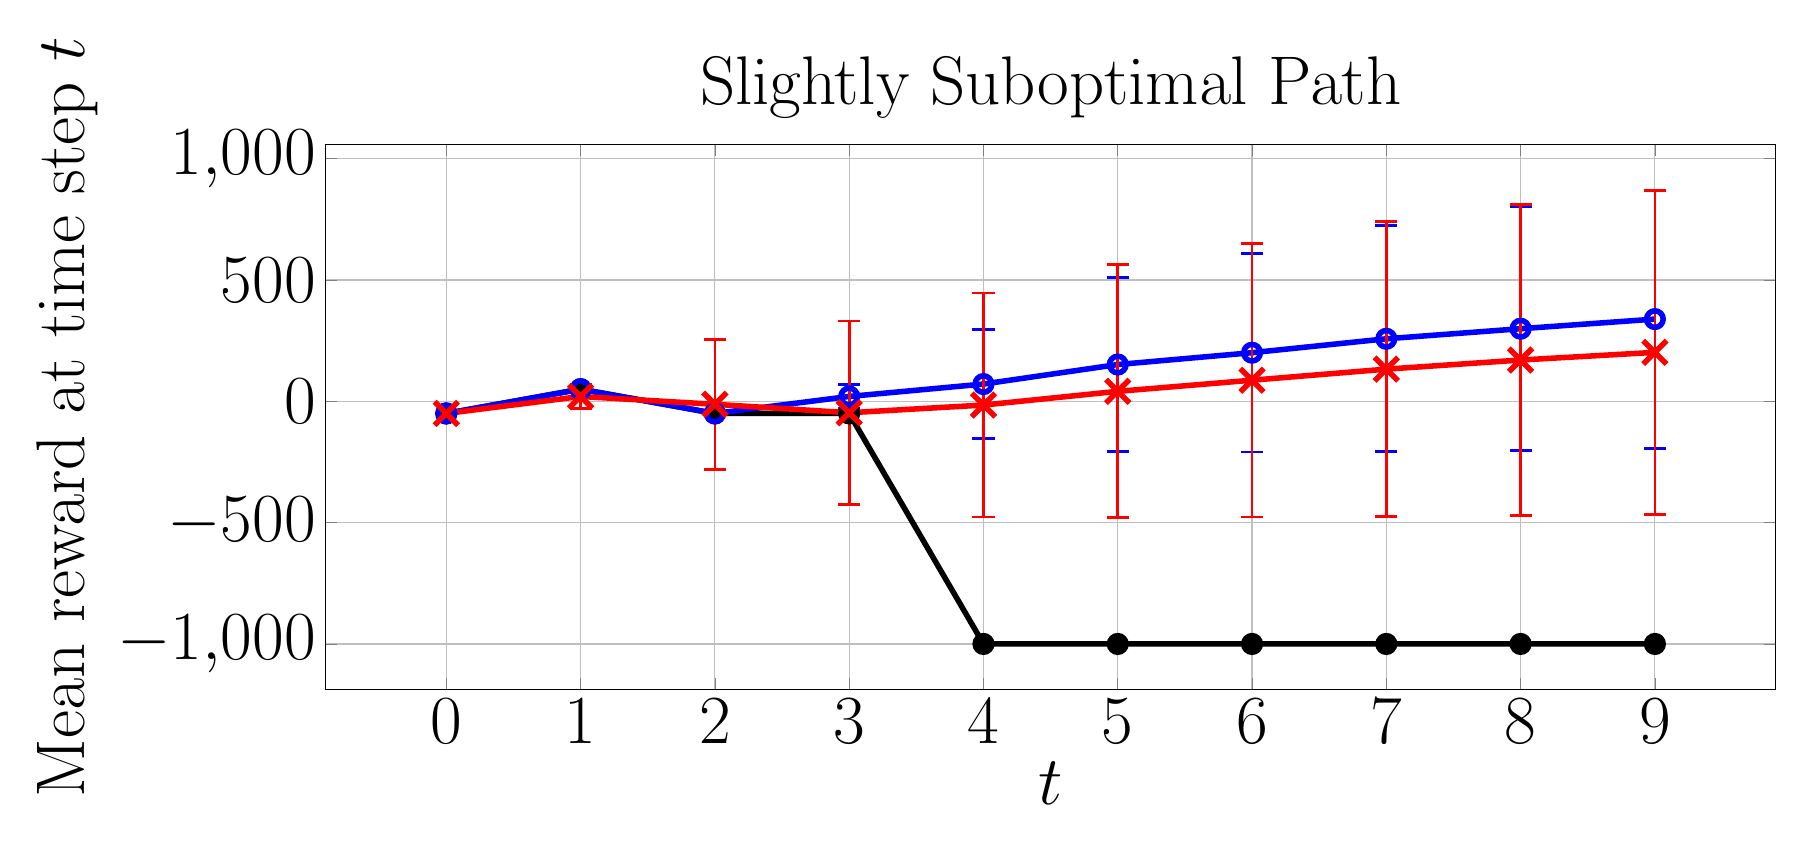
\begin{tikzpicture}
                \begin{axis}[
                    xlabel={$t$},
                    ylabel={Mean reward at time step $t$},
                    title={Slightly Suboptimal Path},
                    grid=both,
                    width=20cm, height=8.5cm,
                    every axis/.style={font=\Huge},
                    %
                ]
               \addplot[
                    color=black, %
                    mark=*, %
                    line width=2pt,
                    mark size=3pt,
                ]
                coordinates {
                    (0, -50.0)
                    (1, 50.0)
                    (2, -50.0)
                    (3, -50.0)
                    (4, -1000.0)
                    (5, -1000.0)
                    (6, -1000.0)
                    (7, -1000.0)
                    (8, -1000.0)
                    (9, -1000.0)
                };
                %
                \addplot[
                    color=blue, %
                    mark=o, %
                    line width=2pt,
                    mark size=3pt,
                    error bars/.cd,
                    y dir=both, %
                    y explicit, %
                    error bar style={line width=1pt,solid},
                    error mark options={line width=1pt,mark size=4pt,rotate=90}
                ]
                coordinates {
                    (0, -50.0)  +- (0, 0.0)
                    (1, 50.0)  +- (0, 0.0) 
                    (2, -50.0)  +- (0, 0.0) 
                    (3, 20.0631)  +- (0, 49.97539413)
                    (4, 71.206585)  +- (0, 226.02033693)
                    (5, 151.60797) +- (0, 359.23292559)
                    (6, 200.40593) +- (0, 408.86185176)
                    (7, 257.77948) +- (0, 466.10372804)
                    (8, 299.237465) +- (0, 501.82579506)
                    (9, 338.9129) +- (0, 532.06124996)
                };
                %
                \addplot[
                    color=red, %
                    mark=x, %
                    line width=2pt,
                    mark size=6pt,
                    error bars/.cd,
                    y dir=both, %
                    y explicit, %
                    error bar style={line width=1pt,solid},
                    error mark options={line width=1pt,mark size=4pt,rotate=90}
                ]
                coordinates {
                    (0, -50.0)  +- (0, 0.0)
                    (1, 20.00736)  +- (0, 49.99786741) 
                    (2, -12.282865)  +- (0, 267.598755) 
                    (3, -47.125995)  +- (0, 378.41755832)
                    (4, -15.381965)  +- (0, 461.77616558)
                    (5, 41.15459) +- (0, 521.53189262)
                    (6, 87.01595) +- (0, 564.22243126 )
                    (7, 132.62376) +- (0, 607.31338037)
                    (8, 170.168145) +- (0, 641.48013693)
                    (9, 201.813135) +- (0, 667.29441777)
                };
                %
                %
                %
                %
                %
                %
                %
                %
                %
                %
                %
                %
                %
                %
                %
                %
                %
                %
                %
                \end{axis}
            \end{tikzpicture}
         }
    }\\[-1.5pt]
    \subfigure[\footnotesize Lowest cumulative reward: Interval CFMDP ($100$), Gumbel-max SCM ($100$)]{%
         \resizebox{0.76\columnwidth}{!}{
             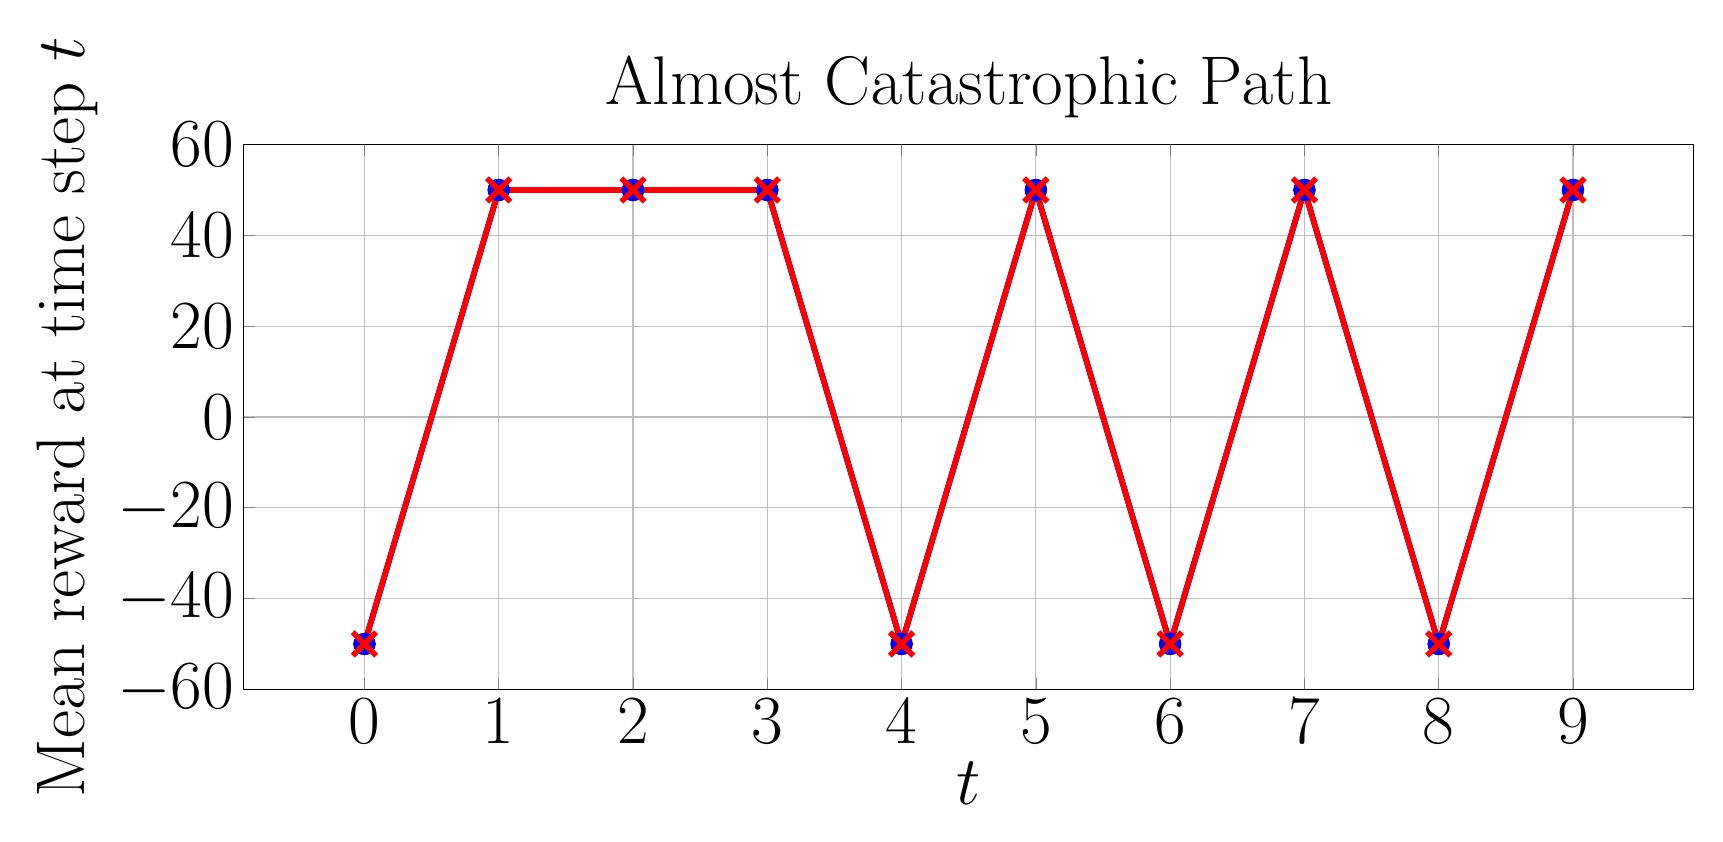
\begin{tikzpicture}
                \begin{axis}[
                    xlabel={$t$},
                    ylabel={Mean reward at time step $t$},
                    title={Almost Catastrophic Path},
                    grid=both,
                    every axis/.style={font=\Huge},
                    width=20cm, height=8.5cm,
                    %
                ]
               \addplot[
                    color=black, %
                    mark=*, %
                    line width=2pt,
                    mark size=3pt,
                ]
                coordinates {
                    (0, -50.0)
                    (1, 50.0)
                    (2, 50.0)
                    (3, 50.0)
                    (4, -50.0)
                    (5, 50.0)
                    (6, -50.0)
                    (7, 50.0)
                    (8, -50.0)
                    (9, 50.0)
                };
                %
                %
                \addplot[
                    color=blue, %
                    mark=o, %
                    line width=2pt,
                    mark size=3pt,
                    error bars/.cd,
                    y dir=both, %
                    y explicit, %
                    error bar style={line width=1pt,solid},
                    error mark options={line width=1pt,mark size=4pt,rotate=90}
                ]
                coordinates {
                    (0, -50.0)  +- (0, 0.0)
                    (1, 50.0)  +- (0, 0.0) 
                    (2, 50.0)  +- (0, 0.0) 
                    (3, 50.0)  +- (0, 0.0)
                    (4, -50.0)  +- (0, 0.0)
                    (5, 50.0) +- (0, 0.0)
                    (6, -50.0) +- (0, 0.0)
                    (7, 50.0) +- (0, 0.0)
                    (8, -50.0) +- (0, 0.0)
                    (9, 50.0) +- (0, 0.0)
                };
                %
                \addplot[
                    color=red, %
                    mark=x, %
                    line width=2pt,
                    mark size=6pt,
                    error bars/.cd,
                    y dir=both, %
                    y explicit, %
                    error bar style={line width=1pt,solid},
                    error mark options={line width=1pt,mark size=4pt,rotate=90}
                ]
                coordinates {
                    (0, -50.0)  +- (0, 0.0)
                    (1, 50.0)  +- (0, 0.0) 
                    (2, 50.0)  +- (0, 0.0) 
                    (3, 50.0)  +- (0, 0.0)
                    (4, -50.0)  +- (0, 0.0)
                    (5, 50.0) +- (0, 0.0)
                    (6, -50.0) +- (0, 0.0)
                    (7, 50.0) +- (0, 0.0)
                    (8, -50.0) +- (0, 0.0)
                    (9, 50.0) +- (0, 0.0)
                };
                %
                %
                %
                %
                %
                %
                %
                %
                %
                %
                %
                %
                %
                %
                %
                %
                %
                %
                %
                \end{axis}
            \end{tikzpicture}
         }
    }
    \hspace{1cm}
    \subfigure[\footnotesize Lowest cumulative reward: Interval CFMDP ($-7150$), Gumbel-max SCM ($-9050$)]{%
         \resizebox{0.76\columnwidth}{!}{
            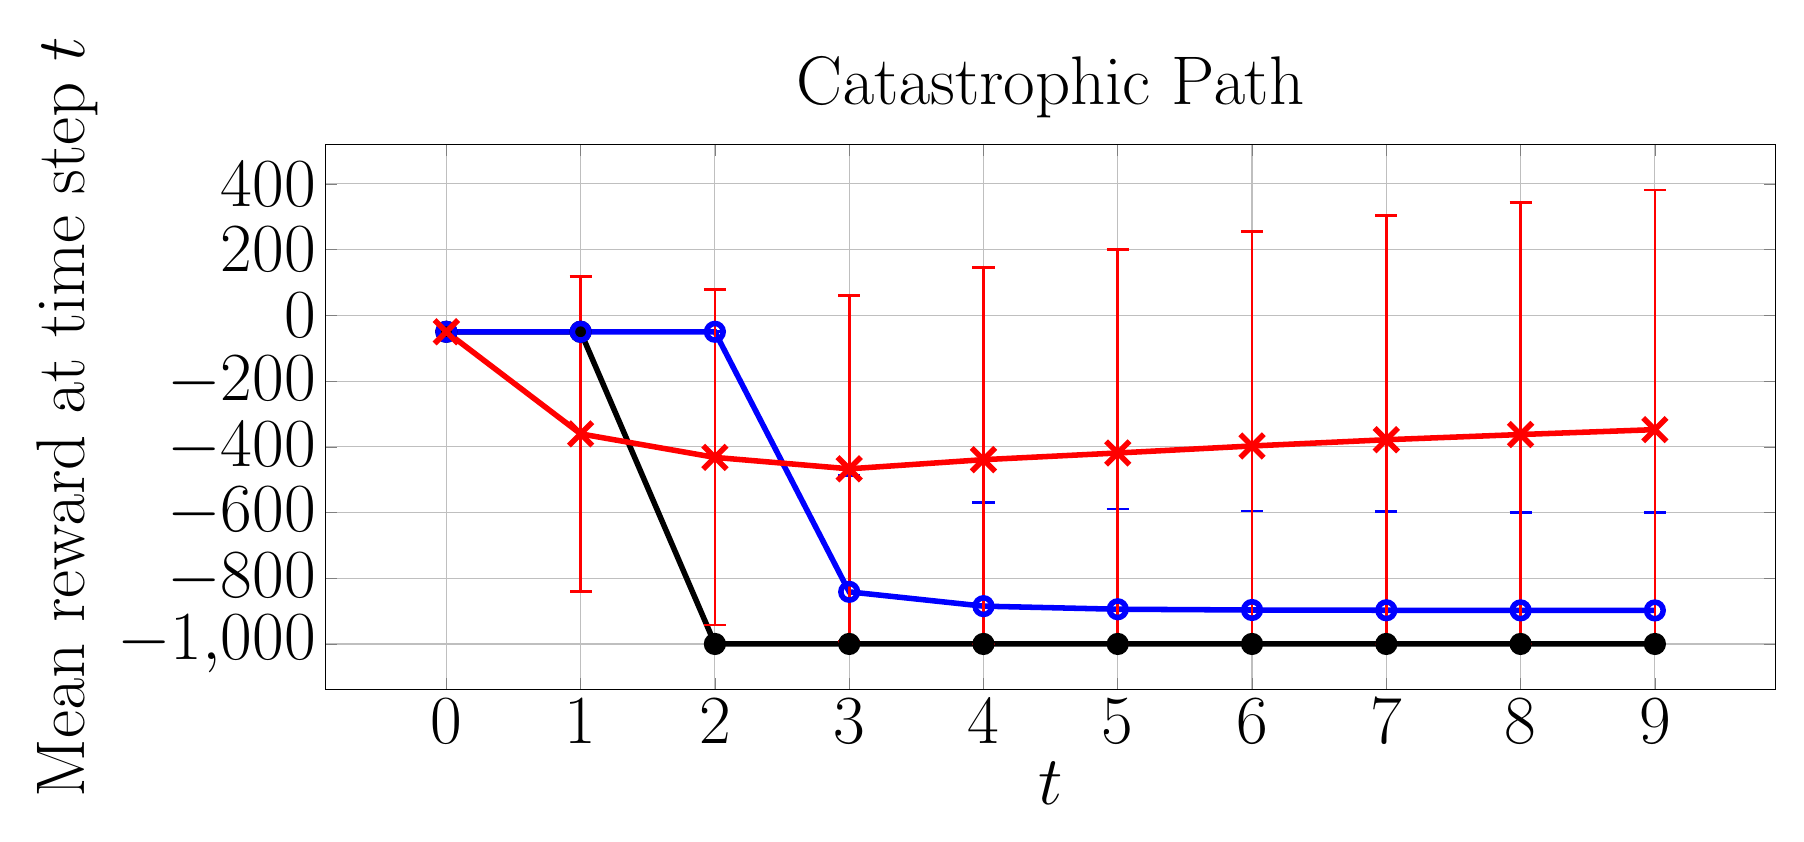
\begin{tikzpicture}
                \begin{axis}[
                    xlabel={$t$},
                    ylabel={Mean reward at time step $t$},
                    title={Catastrophic Path},
                    grid=both,
                    width=20cm, height=8.5cm,
                    every axis/.style={font=\Huge},
                    %
                ]
               \addplot[
                    color=black, %
                    mark=*, %
                    line width=2pt,
                    mark size=3pt,
                ]
                coordinates {
                    (0, -50.0)
                    (1, -50.0)
                    (2, -1000.0)
                    (3, -1000.0)
                    (4, -1000.0)
                    (5, -1000.0)
                    (6, -1000.0)
                    (7, -1000.0)
                    (8, -1000.0)
                    (9, -1000.0)
                };
                %
                %
                \addplot[
                    color=blue, %
                    mark=o, %
                    line width=2pt,
                    mark size=3pt,
                    error bars/.cd,
                    y dir=both, %
                    y explicit, %
                    error bar style={line width=1pt,solid},
                    error mark options={line width=1pt,mark size=4pt,rotate=90}
                ]
                coordinates {
                    (0, -50.0)  +- (0, 0.0)
                    (1, -50.0)  +- (0, 0.0) 
                    (2, -50.0)  +- (0, 0.0) 
                    (3, -841.440725)  += (0, 354.24605512) -= (0, 158.559275)
                    (4, -884.98225)  += (0, 315.37519669) -= (0, 115.01775)
                    (5, -894.330425) += (0, 304.88572805) -= (0, 105.669575)
                    (6, -896.696175) += (0, 301.19954514) -= (0, 103.303825)
                    (7, -897.4635) += (0, 299.61791279) -= (0, 102.5365)
                    (8, -897.77595) += (0, 298.80392585) -= (0, 102.22405)
                    (9, -897.942975) += (0, 298.32920557) -= (0, 102.057025)
                };
                %
                \addplot[
                    color=red, %
                    mark=x, %
                    line width=2pt,
                    mark size=6pt,
                    error bars/.cd,
                    y dir=both, %
                    y explicit, %
                    error bar style={line width=1pt,solid},
                    error mark options={line width=1pt,mark size=4pt,rotate=90}
                ]
            coordinates {
                    (0, -50.0)  +- (0, 0.0)
                    (1, -360.675265)  +- (0, 479.39812699) 
                    (2, -432.27629)  +- (0, 510.38620897) 
                    (3, -467.029545)  += (0, 526.36009628) -= (0, 526.36009628)
                    (4, -439.17429)  += (0, 583.96638919) -= (0, 560.82571)
                    (5, -418.82704) += (0, 618.43027478) -= (0, 581.17296)
                    (6, -397.464895) += (0, 652.67322574) -= (0, 602.535105)
                    (7, -378.49052) += (0, 682.85407033) -= (0, 621.50948)
                    (8, -362.654195) += (0, 707.01412023) -= (0, 637.345805)
                    (9, -347.737935) += (0, 729.29076479) -= (0, 652.262065)
                };
                %
                %
                %
                %
                %
                %
                %
                %
                %
                %
                %
                %
                %
                %
                %
                %
                %
                %
                %
                \end{axis}
            \end{tikzpicture}
         }
    }
    \caption{Average instant reward of CF paths induced by policies on Sepsis.}
    \label{fig: reward sepsis}
\end{figure*}

%
%
%
\subsection{Interval CFMDP Bounds}
%
%
Table \ref{tab:nonzero_probs} presents the mean counterfactual probability bound widths (excluding transitions where the upper bound is $0$) for each MDP, averaged over 20 observed paths. We compare the bounds under counterfactual stability (CS) and monotonicity (M) assumptions, CS alone, and no assumptions. This shows that the assumptions marginally reduce the bound widths, indicating the assumptions tighten the bounds without excluding too many causal models, as intended.
\renewcommand{\arraystretch}{1}

\begin{table}
\centering
\caption{Mean width of counterfactual probability bounds}
\resizebox{0.8\columnwidth}{!}{%
\begin{tabular}{|c|c|c|c|}
\hline
\multirow{2}{*}{\textbf{Environment}} & \multicolumn{3}{c|}{\textbf{Assumptions}} \\ \cline{2-4}
 & \textbf{CS + M} & \textbf{CS} & \textbf{None\tablefootnote{\jl{Equivalent to \citet{li2024probabilities}'s bounds (see Section \ref{sec: equivalence with Li}).}}} \\ \hline
\textbf{GridWorld} ($p=0.9$) & 0.0817 & 0.0977 & 0.100 \\ \hline
\textbf{GridWorld} ($p=0.4$) & 0.552  & 0.638  & 0.646 \\ \hline
\textbf{Sepsis} & 0.138 & 0.140 & 0.140 \\ \hline
\end{tabular}
}
\label{tab:nonzero_probs}
\end{table}


\subsection{Execution Times}
Table \ref{tab: times} compares the average time needed to generate the interval CFMDP vs.\ the Gumbel-max SCM CFMDP for 20 observations.
The GridWorld algorithms were run single-threaded, while the Sepsis experiments were run in parallel.
Generating the interval CFMDP is significantly faster as it uses exact analytical bounds, whereas the Gumbel-max CFMDP requires sampling from the Gumbel distribution to estimate counterfactual transition probabilities. \jl{Since constructing the counterfactual MDP models is the main bottleneck in both approaches, ours is more efficient overall and suitable for larger MDPs.}
\begin{table}
\centering
\caption{Mean execution time to generate CFMDPs}
\resizebox{0.99\columnwidth}{!}{%
\begin{tabular}{|c|c|c|}
\hline
\multirow{2}{*}{\textbf{Environment}} & \multicolumn{2}{c|}{\textbf{Mean Execution Time (s)}} \\ \cline{2-3} 
                                      & \textbf{Interval CFMDP} & \textbf{Gumbel-max CFMDP} \\ \hline
\textbf{GridWorld ($p=0.9$) }                  & 0.261                   & 56.1                      \\ \hline
\textbf{GridWorld ($p=0.4$)  }                 & 0.336                   & 54.5                      \\ \hline
\textbf{Sepsis}                                 & 688                     & 2940                      \\ \hline
\end{tabular}%
}
\label{tab: times}
\end{table}


\begin{tikzpicture}[
	font=\footnotesize,
	node distance=0.3cm
	]
	\node[] (P) at (0,0)  {
		\textbf{Parameter:} Key-Gen()
	};
	\node[] (c) [below = 0cm of P] {
		\begin{minipage}{0.8\columnwidth}
			\begin{minted}[fontsize=\footnotesize,escapeinside=@@,autogobble]{coq}
Parameter KeyGen, (PubKey × SecKey).
			\end{minted}
		\end{minipage}
	};
	
	% Package frame and stuff
	\draw[] (c.north west) |- (P.north) -| (c.north east);
	\draw[] (c.north west) |- (P.south) -| (c.north east);
	\draw[] (c.north east) |- (c.south) -| (c.north west);
	
	%%%%%%%%%%%%%%%%%%%%%%%%%%%%%%%%%%%%%%%
	%%%%%%%%%%%%%%% Sign %%%%%%%%%%%%%%%%%%
	%%%%%%%%%%%%%%%%%%%%%%%%%%%%%%%%%%%%%%%
	
	\node[] (P1) [below = 0.7cm of P]  {
		\textbf{Parameter:} Sign(m,sk)
	};
	\node[] (c1) [below = 0cm of P1] {
		\begin{minipage}{0.8\columnwidth}
			\begin{minted}[fontsize=\footnotesize,escapeinside=@@,autogobble]{coq}
Parameter Sign : @$\forall$@ (sk : SecKey) (m : Message), 
  Signature.
			\end{minted}
		\end{minipage}
	};
	
	% Package frame and stuff
	\draw[] (c1.north west) |- (P1.north) -| (c1.north east);
	\draw[] (c1.north west) |- (P1.south) -| (c1.north east);
	\draw[] (c1.north east) |- (c1.south) -| (c1.north west);
	
	%%%%%%%%%%%%%%%%%%%%%%%%%%%%%%%%%%%%%%%
	%%%%%%%%%%%%%%% Verify %%%%%%%%%%%%%%%%
	%%%%%%%%%%%%%%%%%%%%%%%%%%%%%%%%%%%%%%%
	
	\node[] (P2) [below = 1cm of P1]  {
		\textbf{Parameter:} Verify(m,sig,pk)
	};
	\node[] (c2) [below = 0cm of P2] {
		\begin{minipage}{0.8\columnwidth}
			\begin{minted}[fontsize=\footnotesize,escapeinside=@@,autogobble]{coq}
Parameter Ver_sig : @$\forall$@ (pk : PubKey) 
  (sig : Signature) (m : Message), bool.
			\end{minted}
		\end{minipage}
	};
	
	% Package frame and stuff
	\draw[] (c2.north west) |- (P2.north) -| (c2.north east);
	\draw[] (c2.north west) |- (P2.south) -| (c2.north east);
	\draw[] (c2.north east) |- (c2.south) -| (c2.north west);
	
\end{tikzpicture}


\begin{table*}[t]
\centering
\fontsize{11pt}{11pt}\selectfont
\begin{tabular}{lllllllllllll}
\toprule
\multicolumn{1}{c}{\textbf{task}} & \multicolumn{2}{c}{\textbf{Mir}} & \multicolumn{2}{c}{\textbf{Lai}} & \multicolumn{2}{c}{\textbf{Ziegen.}} & \multicolumn{2}{c}{\textbf{Cao}} & \multicolumn{2}{c}{\textbf{Alva-Man.}} & \multicolumn{1}{c}{\textbf{avg.}} & \textbf{\begin{tabular}[c]{@{}l@{}}avg.\\ rank\end{tabular}} \\
\multicolumn{1}{c}{\textbf{metrics}} & \multicolumn{1}{c}{\textbf{cor.}} & \multicolumn{1}{c}{\textbf{p-v.}} & \multicolumn{1}{c}{\textbf{cor.}} & \multicolumn{1}{c}{\textbf{p-v.}} & \multicolumn{1}{c}{\textbf{cor.}} & \multicolumn{1}{c}{\textbf{p-v.}} & \multicolumn{1}{c}{\textbf{cor.}} & \multicolumn{1}{c}{\textbf{p-v.}} & \multicolumn{1}{c}{\textbf{cor.}} & \multicolumn{1}{c}{\textbf{p-v.}} &  &  \\ \midrule
\textbf{S-Bleu} & 0.50 & 0.0 & 0.47 & 0.0 & 0.59 & 0.0 & 0.58 & 0.0 & 0.68 & 0.0 & 0.57 & 5.8 \\
\textbf{R-Bleu} & -- & -- & 0.27 & 0.0 & 0.30 & 0.0 & -- & -- & -- & -- & - &  \\
\textbf{S-Meteor} & 0.49 & 0.0 & 0.48 & 0.0 & 0.61 & 0.0 & 0.57 & 0.0 & 0.64 & 0.0 & 0.56 & 6.1 \\
\textbf{R-Meteor} & -- & -- & 0.34 & 0.0 & 0.26 & 0.0 & -- & -- & -- & -- & - &  \\
\textbf{S-Bertscore} & \textbf{0.53} & 0.0 & {\ul 0.80} & 0.0 & \textbf{0.70} & 0.0 & {\ul 0.66} & 0.0 & {\ul0.78} & 0.0 & \textbf{0.69} & \textbf{1.7} \\
\textbf{R-Bertscore} & -- & -- & 0.51 & 0.0 & 0.38 & 0.0 & -- & -- & -- & -- & - &  \\
\textbf{S-Bleurt} & {\ul 0.52} & 0.0 & {\ul 0.80} & 0.0 & 0.60 & 0.0 & \textbf{0.70} & 0.0 & \textbf{0.80} & 0.0 & {\ul 0.68} & {\ul 2.3} \\
\textbf{R-Bleurt} & -- & -- & 0.59 & 0.0 & -0.05 & 0.13 & -- & -- & -- & -- & - &  \\
\textbf{S-Cosine} & 0.51 & 0.0 & 0.69 & 0.0 & {\ul 0.62} & 0.0 & 0.61 & 0.0 & 0.65 & 0.0 & 0.62 & 4.4 \\
\textbf{R-Cosine} & -- & -- & 0.40 & 0.0 & 0.29 & 0.0 & -- & -- & -- & -- & - & \\ \midrule
\textbf{QuestEval} & 0.23 & 0.0 & 0.25 & 0.0 & 0.49 & 0.0 & 0.47 & 0.0 & 0.62 & 0.0 & 0.41 & 9.0 \\
\textbf{LLaMa3} & 0.36 & 0.0 & \textbf{0.84} & 0.0 & {\ul{0.62}} & 0.0 & 0.61 & 0.0 &  0.76 & 0.0 & 0.64 & 3.6 \\
\textbf{our (3b)} & 0.49 & 0.0 & 0.73 & 0.0 & 0.54 & 0.0 & 0.53 & 0.0 & 0.7 & 0.0 & 0.60 & 5.8 \\
\textbf{our (8b)} & 0.48 & 0.0 & 0.73 & 0.0 & 0.52 & 0.0 & 0.53 & 0.0 & 0.7 & 0.0 & 0.59 & 6.3 \\  \bottomrule
\end{tabular}
\caption{Pearson correlation on human evaluation on system output. `R-': reference-based. `S-': source-based.}
\label{tab:sys}
\end{table*}



\begin{table}%[]
\centering
\fontsize{11pt}{11pt}\selectfont
\begin{tabular}{llllll}
\toprule
\multicolumn{1}{c}{\textbf{task}} & \multicolumn{1}{c}{\textbf{Lai}} & \multicolumn{1}{c}{\textbf{Zei.}} & \multicolumn{1}{c}{\textbf{Scia.}} & \textbf{} & \textbf{} \\ 
\multicolumn{1}{c}{\textbf{metrics}} & \multicolumn{1}{c}{\textbf{cor.}} & \multicolumn{1}{c}{\textbf{cor.}} & \multicolumn{1}{c}{\textbf{cor.}} & \textbf{avg.} & \textbf{\begin{tabular}[c]{@{}l@{}}avg.\\ rank\end{tabular}} \\ \midrule
\textbf{S-Bleu} & 0.40 & 0.40 & 0.19* & 0.33 & 7.67 \\
\textbf{S-Meteor} & 0.41 & 0.42 & 0.16* & 0.33 & 7.33 \\
\textbf{S-BertS.} & {\ul0.58} & 0.47 & 0.31 & 0.45 & 3.67 \\
\textbf{S-Bleurt} & 0.45 & {\ul 0.54} & {\ul 0.37} & 0.45 & {\ul 3.33} \\
\textbf{S-Cosine} & 0.56 & 0.52 & 0.3 & {\ul 0.46} & {\ul 3.33} \\ \midrule
\textbf{QuestE.} & 0.27 & 0.35 & 0.06* & 0.23 & 9.00 \\
\textbf{LlaMA3} & \textbf{0.6} & \textbf{0.67} & \textbf{0.51} & \textbf{0.59} & \textbf{1.0} \\
\textbf{Our (3b)} & 0.51 & 0.49 & 0.23* & 0.39 & 4.83 \\
\textbf{Our (8b)} & 0.52 & 0.49 & 0.22* & 0.43 & 4.83 \\ \bottomrule
\end{tabular}
\caption{Pearson correlation on human ratings on reference output. *not significant; we cannot reject the null hypothesis of zero correlation}
\label{tab:ref}
\end{table}


\begin{table*}%[]
\centering
\fontsize{11pt}{11pt}\selectfont
\begin{tabular}{lllllllll}
\toprule
\textbf{task} & \multicolumn{1}{c}{\textbf{ALL}} & \multicolumn{1}{c}{\textbf{sentiment}} & \multicolumn{1}{c}{\textbf{detoxify}} & \multicolumn{1}{c}{\textbf{catchy}} & \multicolumn{1}{c}{\textbf{polite}} & \multicolumn{1}{c}{\textbf{persuasive}} & \multicolumn{1}{c}{\textbf{formal}} & \textbf{\begin{tabular}[c]{@{}l@{}}avg. \\ rank\end{tabular}} \\
\textbf{metrics} & \multicolumn{1}{c}{\textbf{cor.}} & \multicolumn{1}{c}{\textbf{cor.}} & \multicolumn{1}{c}{\textbf{cor.}} & \multicolumn{1}{c}{\textbf{cor.}} & \multicolumn{1}{c}{\textbf{cor.}} & \multicolumn{1}{c}{\textbf{cor.}} & \multicolumn{1}{c}{\textbf{cor.}} &  \\ \midrule
\textbf{S-Bleu} & -0.17 & -0.82 & -0.45 & -0.12* & -0.1* & -0.05 & -0.21 & 8.42 \\
\textbf{R-Bleu} & - & -0.5 & -0.45 &  &  &  &  &  \\
\textbf{S-Meteor} & -0.07* & -0.55 & -0.4 & -0.01* & 0.1* & -0.16 & -0.04* & 7.67 \\
\textbf{R-Meteor} & - & -0.17* & -0.39 & - & - & - & - & - \\
\textbf{S-BertScore} & 0.11 & -0.38 & -0.07* & -0.17* & 0.28 & 0.12 & 0.25 & 6.0 \\
\textbf{R-BertScore} & - & -0.02* & -0.21* & - & - & - & - & - \\
\textbf{S-Bleurt} & 0.29 & 0.05* & 0.45 & 0.06* & 0.29 & 0.23 & 0.46 & 4.2 \\
\textbf{R-Bleurt} & - &  0.21 & 0.38 & - & - & - & - & - \\
\textbf{S-Cosine} & 0.01* & -0.5 & -0.13* & -0.19* & 0.05* & -0.05* & 0.15* & 7.42 \\
\textbf{R-Cosine} & - & -0.11* & -0.16* & - & - & - & - & - \\ \midrule
\textbf{QuestEval} & 0.21 & {\ul{0.29}} & 0.23 & 0.37 & 0.19* & 0.35 & 0.14* & 4.67 \\
\textbf{LlaMA3} & \textbf{0.82} & \textbf{0.80} & \textbf{0.72} & \textbf{0.84} & \textbf{0.84} & \textbf{0.90} & \textbf{0.88} & \textbf{1.00} \\
\textbf{Our (3b)} & 0.47 & -0.11* & 0.37 & 0.61 & 0.53 & 0.54 & 0.66 & 3.5 \\
\textbf{Our (8b)} & {\ul{0.57}} & 0.09* & {\ul 0.49} & {\ul 0.72} & {\ul 0.64} & {\ul 0.62} & {\ul 0.67} & {\ul 2.17} \\ \bottomrule
\end{tabular}
\caption{Pearson correlation on human ratings on our constructed test set. 'R-': reference-based. 'S-': source-based. *not significant; we cannot reject the null hypothesis of zero correlation}
\label{tab:con}
\end{table*}

\section{Results}
We benchmark the different metrics on the different datasets using correlation to human judgement. For content preservation, we show results split on data with system output, reference output and our constructed test set: we show that the data source for evaluation leads to different conclusions on the metrics. In addition, we examine whether the metrics can rank style transfer systems similar to humans. On style strength, we likewise show correlations between human judgment and zero-shot evaluation approaches. When applicable, we summarize results by reporting the average correlation. And the average ranking of the metric per dataset (by ranking which metric obtains the highest correlation to human judgement per dataset). 

\subsection{Content preservation}
\paragraph{How do data sources affect the conclusion on best metric?}
The conclusions about the metrics' performance change radically depending on whether we use system output data, reference output, or our constructed test set. Ideally, a good metric correlates highly with humans on any data source. Ideally, for meta-evaluation, a metric should correlate consistently across all data sources, but the following shows that the correlations indicate different things, and the conclusion on the best metric should be drawn carefully.

Looking at the metrics correlations with humans on the data source with system output (Table~\ref{tab:sys}), we see a relatively high correlation for many of the metrics on many tasks. The overall best metrics are S-BertScore and S-BLEURT (avg+avg rank). We see no notable difference in our method of using the 3B or 8B model as the backbone.

Examining the average correlations based on data with reference output (Table~\ref{tab:ref}), now the zero-shoot prompting with LlaMA3 70B is the best-performing approach ($0.59$ avg). Tied for second place are source-based cosine embedding ($0.46$ avg), BLEURT ($0.45$ avg) and BertScore ($0.45$ avg). Our method follows on a 5. place: here, the 8b version (($0.43$ avg)) shows a bit stronger results than 3b ($0.39$ avg). The fact that the conclusions change, whether looking at reference or system output, confirms the observations made by \citet{scialom-etal-2021-questeval} on simplicity transfer.   

Now consider the results on our test set (Table~\ref{tab:con}): Several metrics show low or no correlation; we even see a significantly negative correlation for some metrics on ALL (BLEU) and for specific subparts of our test set for BLEU, Meteor, BertScore, Cosine. On the other end, LlaMA3 70B is again performing best, showing strong results ($0.82$ in ALL). The runner-up is now our 8B method, with a gap to the 3B version ($0.57$ vs $0.47$ in ALL). Note our method still shows zero correlation for the sentiment task. After, ranks BLEURT ($0.29$), QuestEval ($0.21$), BertScore ($0.11$), Cosine ($0.01$).  

On our test set, we find that some metrics that correlate relatively well on the other datasets, now exhibit low correlation. Hence, with our test set, we can now support the logical reasoning with data evidence: Evaluation of content preservation for style transfer needs to take the style shift into account. This conclusion could not be drawn using the existing data sources: We hypothesise that for the data with system-based output, successful output happens to be very similar to the source sentence and vice versa, and reference-based output might not contain server mistakes as they are gold references. Thus, none of the existing data sources tests the limits of the metrics.  


\paragraph{How do reference-based metrics compare to source-based ones?} Reference-based metrics show a lower correlation than the source-based counterpart for all metrics on both datasets with ratings on references (Table~\ref{tab:sys}). As discussed previously, reference-based metrics for style transfer have the drawback that many different good solutions on a rewrite might exist and not only one similar to a reference.


\paragraph{How well can the metrics rank the performance of style transfer methods?}
We compare the metrics' ability to judge the best style transfer methods w.r.t. the human annotations: Several of the data sources contain samples from different style transfer systems. In order to use metrics to assess the quality of the style transfer system, metrics should correctly find the best-performing system. Hence, we evaluate whether the metrics for content preservation provide the same system ranking as human evaluators. We take the mean of the score for every output on each system and the mean of the human annotations; we compare the systems using the Kendall's Tau correlation. 

We find only the evaluation using the dataset Mir, Lai, and Ziegen to result in significant correlations, probably because of sparsity in a number of system tests (App.~\ref{app:dataset}). Our method (8b) is the only metric providing a perfect ranking of the style transfer system on the Lai data, and Llama3 70B the only one on the Ziegen data. Results in App.~\ref{app:results}. 


\subsection{Style strength results}
%Evaluating style strengths is a challenging task. 
Llama3 70B shows better overall results than our method. However, our method scores higher than Llama3 70B on 2 out of 6 datasets, but it also exhibits zero correlation on one task (Table~\ref{tab:styleresults}).%More work i s needed on evaluating style strengths. 
 
\begin{table}%[]
\fontsize{11pt}{11pt}\selectfont
\begin{tabular}{lccc}
\toprule
\multicolumn{1}{c}{\textbf{}} & \textbf{LlaMA3} & \textbf{Our (3b)} & \textbf{Our (8b)} \\ \midrule
\textbf{Mir} & 0.46 & 0.54 & \textbf{0.57} \\
\textbf{Lai} & \textbf{0.57} & 0.18 & 0.19 \\
\textbf{Ziegen.} & 0.25 & 0.27 & \textbf{0.32} \\
\textbf{Alva-M.} & \textbf{0.59} & 0.03* & 0.02* \\
\textbf{Scialom} & \textbf{0.62} & 0.45 & 0.44 \\
\textbf{\begin{tabular}[c]{@{}l@{}}Our Test\end{tabular}} & \textbf{0.63} & 0.46 & 0.48 \\ \bottomrule
\end{tabular}
\caption{Style strength: Pearson correlation to human ratings. *not significant; we cannot reject the null hypothesis of zero corelation}
\label{tab:styleresults}
\end{table}

\subsection{Ablation}
We conduct several runs of the methods using LLMs with variations in instructions/prompts (App.~\ref{app:method}). We observe that the lower the correlation on a task, the higher the variation between the different runs. For our method, we only observe low variance between the runs.
None of the variations leads to different conclusions of the meta-evaluation. Results in App.~\ref{app:results}.
\subsection{Online retrieval}

% 1. 介绍motivation和整体步骤
% 2. 检索步骤
% 3. 生成步骤

%Our ArchRAG is a cost-efficient generation method designed to support both specific QA and abstract QA tasks.
%
In the online retrieval phase, after obtaining the query vector for a given question, ArchRAG generates the final answer by first conducting hierarchical search on the C-HNSW index, and then analyzing and filtering of retrieved information.

\subsubsection{Hierarchical search.} 
\label{sec:search}
% 
We first introduce the query process of C-HNSW and then describe the hierarchical search.
%
The query process is the core of C-HNSW, which can be used for constructing C-HNSW as illustrated in Algorithm \ref{alg:query}.

\begin{algorithm}[ht]
  \caption{{C-HNSW query}}
  \label{alg:query}
  \small
   \SetKwInOut{Input}{input}\SetKwInOut{Output}{output}
    \Input{$\mathcal{H} = ({\mathcal G},{L_{inter}})$, $q$, $k$, $l$.}
    % \Output{$k$ Nearest neighbor found by C-HNSW.}
    $s\gets $ a random node in the highest layer $L$\;
    \For{$i \gets L,\cdots,l+1$}{
        $c\gets$ SearchLayer(${ G_i}=(V_i,E_i), q, s, 1, i$)\;
        % $s\gets$ get the nearest node from $K$\;
$s\gets$ find the node in layer $i-1$ via the inter-layer links of $c$\;
    }
    $K\gets$ SearchLayer(${ G_l}=(V_l,E_l), q, s, k, l$)\;
    \Return{$K$;}
    
    \textbf{Procedure} SearchLayer(${G_i}=(V_i,E_i), q, s,k,i$)\;
    $V\gets \{s\}$,  $R\gets \{s\}$, $Q\gets $ initialize a queue containing $s$\; 
    \While{$|R|>0$}{
        $c \gets$ nearest node in $Q$\;
        $f \gets$ furthest node in $R$\;
        \lIf{$d(c,q)>d(f,q)$}{
            {\bf break}
        } 
        \For{each neighbor $x\in N(c)$ in $G_i$}{
            \lIf{$x \in V$}{\textbf{continue}}
            $V\gets V \cup \{x\}$\;
            $f \gets$ furthest node in $R$\;
            \If{$d(x,q)<d(f,q)$\text{ or }$|R|<k$ }{
                $Q\gets Q\cup \{x\}$, $R\gets R\cup \{x\}$\;
                \lIf{$|R|>k$}{remove $f$ from $R$}
            }
        }
    }
        
    \Return{${R}$;}
\end{algorithm}

Specifically, given a specified query layer $l$, query point $q$, and the number $k$ of nearest neighbors, the query algorithm can be implemented through the following iterative process:
\begin{enumerate}
    \item Start from a random node at the highest layer $L$, which serves as the starting node for layer $L$ (line 1).
    
    \item For each layer from layers $L$ to $l+1$, begin at the starting node and use a greedy traversal approach (i.e., the procedure SearchLayer) to find the nearest neighbor $c$ of $q$, and then traverse to the next layer using $c$'s inter-layer link as the starting node for the next layer (lines 2-4).
    
    \item In the query layer $l$, use the greedy traversal approach to find the $k$ nearest neighbors of $q$ (line 5).
\end{enumerate}

Specifically, the greedy traversal strategy compares the distance between the query point and the visited nodes during the search process.
% 
It achieves this by maintaining a candidate expansion queue $Q$ and a dynamic nearest neighbor set $R$, which contains $k$ elements:

\begin{itemize}
    \item Expansion Queue $Q$: For each neighbor $x$ of a visited node, if $d(x,q)<d(f,q)$, where $f$ is the furthest node from $R$ to $q$, then $x$ is added to the expansion queue.
    \item Dynamic Nearest Neighbor Set $R$: Nodes added to $C$ are used to update $R$, ensuring that it maintains no more than $k$ elements, where $k$ is the specified number of query results.
\end{itemize}

In the greedy traversal, if a node $x$ expanded from $Q$ satisfies $
d(n,q)>d(n,f)$, where $f$ is the furthest node from $R$ to $q$, then the traversal stops.


Based on the discussions above, we propose a hierarchical search approach, which retrieves the top $k$ relevant elements in each layer using the method outlined in Algorithm \ref{alg:query}.
% 
% We leverage the C-HNSW index and the C-HNSW query algorithm to retrieve the top $k$ nearest neighbors at each level, starting from the top layer.
% 
Once the query at a given layer is complete, we use the inter-layer link of the nearest neighbor in that layer to traverse to the next layer, repeating the process until reaching the bottom layer.
% 
At the bottom layer, we extract the relationships between connected retrieved entities, forming the text information $R_0$ for this subgraph.
% 
We represent the retrieved information from each layer as $R_i$, where $i \in \{0,1,\cdots, L\}$, to be used in the adaptive filtering-based generation process.

% C-HNSW leverages the structure of hierarchical communities and entities to efficiently query the most relevant information at any layer, including both communities and entities.
% % 
% At each layer, we select the top-k communities or entities most relevant to the query embedding to address queries with varying levels of detail.
% % 
% Specifically, starting from any point in the top layer, we progressively traverse and search, maintaining the nearest neighbor queue.
% 



\subsubsection{Adaptive filtering-based generation. }
While some optimized LLMs support longer text inputs, they may still encounter issues such as the ``lost in the middle'' dilemma \cite{liu2024lost}. 
% 
Thus, direct utilization of retrieved information comprising multiple text segments for LLM-based answer generation risks compromising output accuracy.

To mitigate this limitation, we propose an adaptive filtering-based method that harnesses the LLM’s inherent reasoning capabilities.
% 
We first prompt the LLM to extract and generate an analysis report from the retrieved information, identifying the parts that are most relevant to answering the query and assigning relevance scores to these reports.
% 
Then, all analysis reports are integrated and sorted, ensuring that the most relevant content is used to summarize the final response to the query, with any content exceeding the text limit being truncated.
% 
This process can be represented as:
\begin{align}
A_i &= LLM(P_{filter}||R_i) \\
Output&=LLM(P_{merge}||Sort(\{A_0,A_1,\cdots,A_n\}))
\end{align}
where $P_{filter}$ and $P_{merge}$ represent the prompts for extracting relevant information and summarizing, respectively, 
$A_i$, $i \in 0 \cdots n$ denotes the filtered analysis report.
% 
The sort function orders the content based on the relevance scores from the analysis report. 

We also analyze the complexity of ArchRAG in Appendix \ref{sec:complexity}.

% The Map-Reduce Analysis Generation approach enables the LLM to efficiently utilize a greater amount of retrieved information, leading to more accurate responses and summaries.
% % 
% By minimizing the number of LLM calls and leveraging the LLM's analytical reasoning, a more powerful RAG framework is achieved.
% \section{Computational complexity}\label{sec:compl}

In this section, we show that both of our problems are \np-hard.
We saw in the previous section that if
we set $\alpha  = \infty$, then \problemcdcsm reduces to \problemdts, which can be solved exactly in
polynomial time. However, \problemcdcsm is \np-hard when $\alpha = 0$.
%However, we show next that the complexity of fair densestsubgraph $\problemcdcsm$ which allows $0 < \alpha \leq 1$ is $\np$-hard.


\begin{proposition} 
\label{prop:np}
\problemcdcsm is \np-hard.
\end{proposition} 
\begin{proof}
We prove the hardness from $k$-\prbclique, a problem where, given a graph $H$, we are asked if there is a clique of size at least $k$.

Assume that we are given a graph $H = (V, E)$ with $n$ nodes, $n \geq k$. We set $\alpha = 0$.
The graph snapshot $G_1$ consists of the
graph $H$ and an additional set of $k$ singleton vertices $U$. $G_2$ consists of a $k$-clique connecting the vertices in $U$. 

We claim that there is a subset $S$ yielding $\dens{S, \calG} =  (k - 1)/2$ if and only if there is an $k$-clique in $H$.

Assume that  there is a subset $S$ yielding $\dens{S, \calG} =  (k - 1)/2$.
Since the value of objective is $(k - 1)/2$, we have $\dens{S, G_1} = \dens{S, G_2} = (k - 1)/4$. 
Let $S = W \cup T$ where $W \subseteq V$ and denotes the subset of vertices from $H$ and $T \subseteq U$ is the subset of vertices from  $U$ in $S$. 

Assume that $\abs{W} < \abs{T}$. Since $\abs{T} \leq k$, $\abs{W} < k$.  The density induced on $G_1$ is bounded by $\dens{S, G_1} \leq \frac{{\abs{W} \choose 2}}{\abs{T} + \abs{W}} < \frac{{\abs{W} \choose 2}}{2\abs{W}} < \frac{k - 1}{4}$, which is a contradiction.
Assume that  $\abs{W} > \abs{T}$. Then the density induced on $G_2$ is bounded by $\dens{S, G_2} = \frac{{\abs{T} \choose 2}}{\abs{T} + \abs{W}} < \frac{{\abs{T} \choose 2}}{2\abs{T}} = \frac{\abs{T} - 1}{4} \leq \frac{k - 1}{4}$, again a contradiction. Therefore, $\abs{W} =  \abs{T}$. 

Consequently, $\dens{S, G_2} = (\abs{T} - 1)/4$, implying that $\abs{T} = k$. Finally, $\frac{k - 1}{4} = \dens{S, G_1} = \frac{\abs{E(S)}}{2k}$ implies that $\abs{E} = {k \choose 2}$, that is, $W$ is a $k$-clique in $H$.

%Let  $d_1$ and $d_2$ are the densities induced on $G_1$ and $G_2$ respectively by $S$.
%Based on our assumption, $\dens{S, \calG} =  (k - 1)/2$ yields and 
%the only way to obtain a density value  of $f(S, G_2) = (k - 1)/4$  which satisfies marginal density constraint is that  $S = W \cup U$ and thus there should be an $k$-clique in $H$.
%Therefore, if the density is $  (k - 1)/4$ there is an $k$-clique in $H$.


On the other hand, assume there is a clique $C$ of size $k$ in $H$.
%Let clique $C$ is formed by the set of vertices in $W$.
% Let $d_1$ and $d_2$ are the optimal densities induced on $G_1$ and $G_2$.
% Since the density constraint should be satisfied $d_1 \geq (d_1 + d_2)/2$ and $d_2 \geq (d_1 + d_2)/2$ which implies $d_1 \geq d_2$ and $d_2 \geq d_1$. Therefore, $d_1 = d_2$.  
% Let $k_1$ and $k_2$ number of non-singleton nodes contribute for $d_1$ and $d_2$ respectively.
% Since $d_1 = d_2$,  $\frac{ k_1(k_1 - 1)}{ 2(k_1 + k_2)} = \frac{k_2 (k_2 - 1)}{ 2(k_1 + k_2)}$ which implies $k_1 =  k_2$. Then  the sum of the densities is given by $\frac{ (k_1 - 1)}{ 2} $ where the optimal is  when $k_1  = k =  k_2$.
Set $S = C \cup U$. 
Immediately, $\dens{S, \calG} =   (k - 1)/2$ proving the claim.
\qed
\end{proof}

\iffalse
\begin{proposition}
\label{prop:inapproximability}
\problemcdcsm does not have any polynomial time approximation algorithm with an approximation ratio better than $n^{1-\epsilon}$ for any constant $\epsilon > 0$, unless $\np = \zpp$.
\end{proposition}
\fi

A similar proof will show that \problemcdcsdiff is \np-hard, and inapproximable.

\begin{proposition} 
\label{prop:np2}
\problemcdcsdiff is \np-hard.
Unless $\poly = \np$, there is no polynomial-time algorithm with multiplicative approximation guarantee for \problemcdcsdiff. 
\end{proposition} 

\begin{proof}
We use the same reduction from $k$-\prbclique as in the proof of Proposition~\ref{prop:np}.
We also set $\sigma = (k - 1)/2$. If there is a clique $C$ in $H$, then selecting $S = C \cup U$ yields $\diff{S, \calG} = 0$.
On the other hand, if $\diff{S, \calG} = 0$, then $\dens{S, G_1} = \dens{S, G_2} = (k - 1)/4$, and the argument in the proof of Proposition~\ref{prop:np} shows that there must be a $k$-clique in $H$.
In summary, the difference $\diff{S, \calG} = 0$ for a solution $S$ if and only if there is a $k$-clique in $H$.

This also immediately implies that there is no polynomial-time algorithm with multiplicative approximation guarantee since this algorithm can be then used to test whether there is a set $S$ with $\diff{S, \calG} = 0$.
\qed
\end{proof}



% \textbf{Motivation. } 
% Communities, which represent dense clusters of nodes within a graph network, have been widely applied across various domains \cite{dudleyExploitingDrugdiseaseRelationships2011,pesantez-cabreraEfficientDetectionCommunities2019,fortunatoCommunityDetectionGraphs2010,fangSurveyCommunitySearch2019,fortunatoCommunityDetectionNetworks2016,newmanFindingEvaluatingCommunity2004}. 
% % 
% Motivated by the ability of communities to capture both key information and provide a global perspective, we adopt an attributed community method.
% % 
% The lower-level communities and original node information contain detailed information from the KG, and the higher-level communities provide global summaries, enabling the framework to address both fine-grained specific questions and global abstract questions.
% % 
% Moreover, since only a small portion of the information in a query is relevant, we retrieve only the pertinent data at each layer and analyze it using the LLM, merging the information that satisfies the task requirements.
% % 
% This approach makes ArchRAG highly cost-efficient while integrating data across various granularities and adapting to questions of different levels of detail.



% by splitting the text into chunks and extracting entities and relations from the documents.
% % 
% Based on the KG, we iteratively perform attributed clustering and use an LLM to generate summaries for each community.
% 
% Finally, leveraging the attributed community structure, we construct C-HNSW to support the efficient retrieval of the most relevant community and entity information at each layer.

% During online retrieval, C-HNSW is utilized to search for the most relevant content related to the query at each layer.
% % 
% We then retrieve the most relevant communities and entities from C-HNSW for the query. 
% % 
% To leverage the analytical reasoning capabilities of the LLM, we adopt a Map-Reduce generation approach.
% % 
% In each map executor, the retrieved information is analyzed for relevant content that can assist in answering the query, and all the content is subsequently integrated to generate the final answer.


% In practice, RAG systems receive numerous query requests, and excessive retrieval of content can increase the generation load on the LLM, reducing the accuracy of the responses. 
% 
% Therefore, retrieving relevant content and leveraging large models for reasoning are critical steps in the RAG process.
% 


